%% SCOUT-FL : Sensing-aware Client Selection for Integrated Sensing and Communication
%% Over-the-Air Federated Learning.  Built on the IEEE bare_jrnl (IEEEtran) template.
%% Compiles with pdfLaTeX / tectonic.  Figures live in ./figures as PDF.
\documentclass[lettersize,journal]{IEEEtran}

\usepackage{amsmath,amsfonts,amssymb}
\usepackage{amsthm}
\usepackage{algorithmic}
\usepackage{algorithm}
\usepackage{array}
\usepackage{booktabs}
\usepackage{textcomp}
\usepackage{stfloats}
\usepackage{url}
\usepackage{graphicx}
\usepackage{bm}
\usepackage{cite}
\hyphenation{op-tical net-works semi-conduc-tor IEEE-Xplore}

\graphicspath{{figures/}}

\newtheorem{proposition}{Proposition}
\newtheorem{remark}{Remark}
% IEEE-style end-of-proof marker: filled square on the final line of each proof
% (replaces amsthm's default hollow open box).
\renewcommand{\qedsymbol}{$\blacksquare$}

\newcommand{\R}{\mathbb{R}}
\newcommand{\bw}{\bm{w}}
\newcommand{\bJ}{\bm{J}}
\newcommand{\bg}{\bm{g}}
\newcommand{\calS}{\mathcal{S}}
\newcommand{\calT}{\mathcal{T}}
\newcommand{\calN}{\mathcal{N}}
\newcommand{\calM}{\mathcal{M}}
\newcommand{\calD}{\mathcal{D}}
\newcommand{\tr}{\operatorname{tr}}
\newcommand{\logdet}{\log\det}
\newcommand{\scout}{SCOUT-FL}

\begin{document}

\title{SCOUT-FL: Sensing-Aware Client Selection for\\ Integrated Sensing and Communication\\ in Over-the-Air Federated Learning}

\maketitle

\begin{abstract}
In integrated sensing and communication (ISAC) systems, the transmissions that carry federated learning (FL) updates also illuminate the surrounding targets. The per-round client selection determines both the convergence of the learned model and the sensing quality of the network. Most FL schedulers optimise only the former. This paper presents Sensing-aware Client selection for Over-the-air Uplink Training in Federated Learning (\scout{}), a client-selection rule that treats sensing as a first-class objective. A candidate active set is scored by a monotone submodular utility that couples a diversity-based learning term with a sensing term derived from the per-target Fisher information matrix. The over-the-air aggregation error is kept within a prescribed budget by a lightweight primal--dual price rather than a hard gate. The scheduler thus realises a cognitive cycle of observation, decision, action, and adaptation. Greedy selection attains the $(1-1/e)$ guarantee with a curvature refinement. The dual loop is feasible in time average and incurs no regret and a convergence bound ties the budget to the quality of the trained model. Across a factorial campaign against eleven sensing-aware baselines, \scout{} lies on the accuracy versus Cram\'er--Rao bound Pareto frontier in $96\%$ of operating points and improves final accuracy over the two strongest competitors at one-seventh of the overhead of a recent state-of-the-art scheduler.
\end{abstract}

\begin{IEEEkeywords}
Cognitive networking, integrated sensing and communication, federated learning, over-the-air computation, client selection, submodular optimisation.
\end{IEEEkeywords}

% ============================================================= I. INTRODUCTION
\section{Introduction}
\IEEEPARstart{M}{odern} wireless networks are increasingly required to support communication and environmental sensing with shared spectral and hardware resources. Integrated sensing and communication (ISAC) reuses the same waveform, band, and hardware both to convey information and to probe the physical environment, so that a base station can, within a single transmission, aggregate data from its clients and estimate the range and bearing of surrounding targets~\cite{liu2022isac,cui2021isac}. In parallel, federated learning (FL) has become the standard approach for training a model across many devices without collecting their raw data at the server~\cite{mcmahan2017fedavg}. Over-the-air computation (AirComp) connects the two paradigms. Clients transmit their local model updates simultaneously over a shared multiple-access channel, and the superposition of those signals directly realises the aggregate required by the server \cite{an2026otafl}. The uplink that carries the learning update is thus the same uplink whose echoes carry the sensing information.

This coupling makes the per-round scheduling decision consequential for both tasks. In each communication round the server can activate only a small subset of clients, since power, bandwidth, and latency budgets preclude full participation. The chosen subset determines both the learning signal that reaches the model and the geometry of the sensing measurement, because only the active clients illuminate the targets. A subset whose data is informative but whose radio lines of sight share a common bearing improves the model while leaving the environmental estimate poorly conditioned, whereas a subset spread across bearings sharpens sensing, possibly at some cost to the learning update. The scheduler therefore implicitly negotiates a trade-off between two quantities expressed in different units, namely test accuracy and estimation error.

This negotiation is naturally viewed through the lens of cognitive networking. A cognitive system observes its radio environment, decides under uncertainty, acts, and then learns from the outcome of its own action, following the classical perception and action cycle of cognitive radio~\cite{mitola1999,haykin2005}. The scheduler proposed in this paper instantiates that cycle at the scheduling layer of an ISAC network. In every round it perceives the channel gains, the client geometry, and the gradient embeddings of the clients. It decides the active set through a greedy maximisation. It acts by triggering the joint learning and sensing transmission. It finally learns by updating a dual price from the aggregation error that the transmission actually incurred. The dual price is the memory of the loop, encoding how tight the budget has recently been and reshaping the next decision, much as a cognitive radio adapts its strategy from sensed feedback~\cite{bkassiny2013}. The same cycle continues to organise current designs, from cognitive radios that allocate subcarriers jointly to communication and sensing~\cite{galappaththige2026} to cognition-driven schedulers that adapt client participation in federated edge networks~\cite{lai2026cognition}. The analysis in Section~\ref{sec:theory} makes this loop rigorous. The adaptation is provably feasible in time average, it incurs no regret, and it converts the prescribed error budget into an explicit bound on the learning performance.

\subsection{Related Work and Motivation}
Client selection in FL is a mature topic. Schedulers have been designed around gradient diversity~\cite{balakrishnan2022divfl}, channel state and energy~\cite{yang2020energy,amiri2021scheduling}, combined statistical and system utility~\cite{lai2021oort}, fairness across clients~\cite{li2020fairfl}, and cognition-driven participation control that adapts scheduling to client state online~\cite{lai2026cognition}. The application of submodular utility functions has also been extended to address the representativity of device scheduling in wireless FL~\cite{chen2024exploring}, establishing a precedent for leveraging submodular maximisation to balance wireless resource constraints against learning-centric selection objectives. These approaches share a single-objective formulation in which the sensed environment does not enter the selection criterion. On the ISAC side, a substantial literature co-designs the transmit waveform and beamformer so that one signal serves communication and sensing simultaneously~\cite{liu2020beamforming}, with recent designs driven directly by the Cram\'er--Rao bound of the sensing task~\cite{wang2024cramer,zhou2026crb}, cognitive radio formulations that allocate spectrum jointly to the two functions~\cite{galappaththige2026}, and learning-driven controllers for ISAC resource allocation~\cite{jiang2026marl}. Recent work has further begun to incorporate sensing quality into FL resource allocation and scheduling~\cite{wen2023isacfl,zheng2024otafliscc,du2024fediscc,wen2025isccairfeel,zhang2026isccfl,asaad2025}. The scheduler of Asaad~\emph{et~al.}~\cite{asaad2025}, which prunes a sensing-driven client subset under a combined aggregation-MSE and target-CRB metric, is the closest published point of comparison and serves as the state-of-the-art reference throughout this paper. \\
Recent ISAC-FL frameworks also add orthogonal constraints such as differential privacy \cite{hu2025differentially}. DP mechanisms inject noise into the local updates and change the convergence dynamics, so benchmarking non-private schedulers against DP-constrained methods would be asymmetric. The evaluation pool is therefore restricted to methods under equivalent privacy assumptions.
Three gaps remain. First, sensing quality is usually reduced to a scalar signal-to-noise ratio (SNR) proxy, which neglects the fact that two clients observing a target from the same bearing contribute almost no additional information regardless of their received signal strength. Second, the aggregation-error constraint imposed by AirComp is often enforced by a hard feasibility gate, which is brittle in the sense that a single infeasible round forces the scheduler to discard an otherwise strong candidate set. Third, sensing-aware schedulers are frequently benchmarked against learning-only baselines. A learning-only method is free to disregard sensing entirely and can consequently attain an accuracy that a sensing-aware method correctly declines to pursue. Such comparisons obscure the relevant question, namely how effectively a scheduler trades accuracy against sensing relative to other methods that also carry a sensing objective.

\subsection{Contributions}
This paper proposes \scout{} (Sensing-aware Client selection for Over-the-air Uplink Training in Federated Learning) and evaluates it against sensing-aware baselines exclusively. The contributions are as follows.
\begin{itemize}
\item \textbf{A geometry-aware sensing utility.} A candidate active set is scored by the log-determinant of the aggregate per-target Fisher information matrix (FIM), assembled from an anisotropic per-client FIM that separates radial (range) from tangential (angle) information. Under this utility, angular diversity rather than raw SNR determines the sensing value of a set, and the utility is monotone and submodular (Section~\ref{sec:formulation}).
\item \textbf{A cognitive primal--dual aggregation-MSE constraint.} \scout{} maintains the AirComp aggregation MSE within a budget through a dual variable that ascends on the realised violation, rather than through a hard gate. The update closes a full cognitive cycle of observation, decision, action, and adaptation. The running-average violation is shown to vanish and a no-regret bound is established (Section~\ref{sec:theory}). A convergence result further ties the budget $\varepsilon$ to the quality of the trained model (Proposition~\ref{prop:learn}), so the adaptive price provably converts the constraint into a learning guarantee. The loop is also exercised dynamically. A mid-run budget cut is absorbed within two rounds and the realised error then tracks the new budget in time average (Section~\ref{sec:adapt}). The hard-gate variant is retained as an ablation, denoted \scout{}$^{\dagger}$.
\item \textbf{A characterised greedy guarantee.} The composite learning-plus-sensing utility is monotone submodular, so greedy selection is $(1-1/e)$-optimal with respect to it, and a curvature refinement sharpens the constant (Remark~\ref{rem:curvature}). The bound covers the utility but not the aggregation-MSE penalty, which is min-based and non-submodular. Section~\ref{sec:theory} states precisely which guarantees hold in the slack and binding regimes.
\item \textbf{A sensing-aware evaluation.} Across a factorial campaign spanning data heterogeneity, channel model, SNR, and target geometry, and against eleven sensing-aware baselines, \scout{} is Pareto-optimal on the accuracy--CRB plane in $96\%$ of operating points under both CRB conventions (Fig.~\ref{fig:gapdist}), and attains the highest accuracy of any method that remains inside the sensing-competitive band (Section~\ref{sec:results}).
\end{itemize}
The remainder of the paper is organised as follows. Section~\ref{sec:system} develops the system model, Section~\ref{sec:formulation} states the optimisation problem, Section~\ref{sec:algorithm} presents the \scout{} algorithm, Section~\ref{sec:theory} provides its analysis, Section~\ref{sec:results} reports the numerical study, and Section~\ref{sec:conclusion} concludes the paper.

% ============================================================= II. SYSTEM MODEL
\section{System Model}\label{sec:system}
We consider the ISAC-FL network of Fig.~\ref{fig:system}, comprising a single base station (BS) that also acts as the edge server, a set $\calN=\{1,\dots,N\}$ of clients, and a set $\calM=\{1,\dots,M\}$ of physical targets to be localised. Time is organised into communication rounds $t=1,\dots,T$. In each round the server activates a subset $\calS_t\subseteq\calN$ with $|\calS_t|=K\ll N$, referred to as the \emph{active set}. The clients in the active set transmit their local model updates over the shared uplink, and the same transmissions illuminate the targets and return echoes that the BS uses for sensing.

\begin{figure*}[!t]
\centering
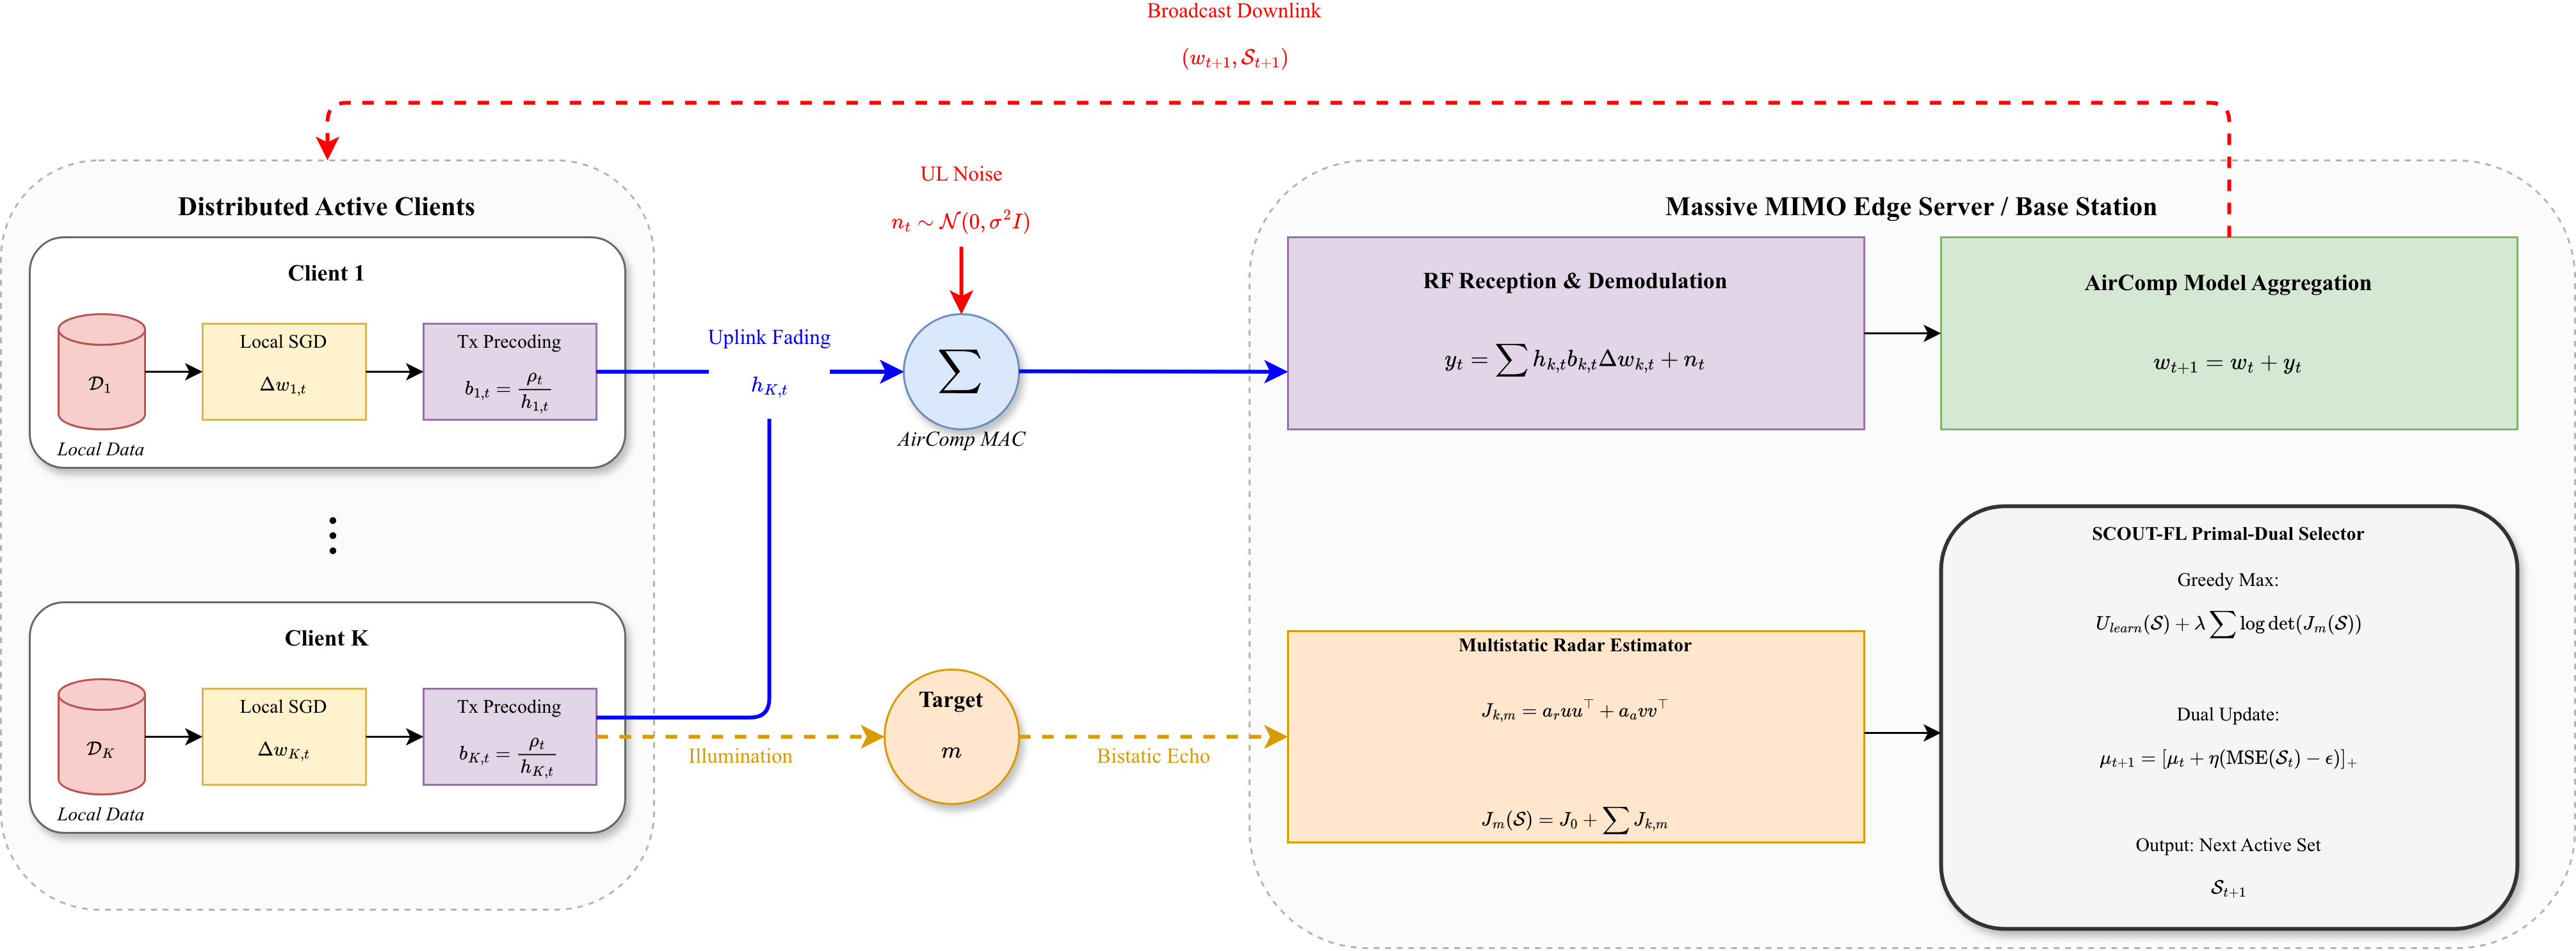
\includegraphics[width=\textwidth]{sys_model.png}
\caption{System model of \scout{}. Each active client performs local SGD, applies channel-inversion precoding $b_{k,t}=\rho_t/h_{k,t}$, and transmits over the shared uplink. The AirComp superposition realises the model aggregate $\bw_{t+1}=\bw_t+\bm{y}_t$ directly, corrupted only by receiver noise, while the same transmissions illuminate the targets and the bistatic echoes assemble the per-target Fisher information $\bJ_m(\calS)$ from the anisotropic contributions~\eqref{eq:fim}. The primal--dual selector greedily maximises the composite utility and updates the dual price $\mu$ on the realised aggregation MSE.}
\label{fig:system}
\end{figure*}

\subsection{Learning Model}
Client $k$ holds a private dataset $\calD_k$ drawn from a client-specific distribution. Heterogeneity across clients is controlled by a Dirichlet concentration parameter $\alpha$, where small $\alpha$ yields strongly non-independent and non-identically distributed (non-IID) partitions. The server maintains a global model $\bw_t\in\R^d$. Given the active set $\calS_t$, each client $k\in\calS_t$ performs local stochastic gradient descent (SGD) from $\bw_t$ and returns an update $\Delta\bw_{k,t}=\bw_{k,t}-\bw_t$. The server forms the aggregate
\begin{equation}
\bw_{t+1}=\bw_t+\sum_{k\in\calS_t} p_{k,t}\,\Delta\bw_{k,t},
\qquad \sum_{k\in\calS_t}p_{k,t}=1,
\label{eq:agg}
\end{equation}
with aggregation weights $p_{k,t}\ge 0$.
Personalised federated strategies keep client-specific models and therefore require the server to access individual updates. AirComp instead yields a single global aggregate through the physical superposition of analog waveforms, so the global model paradigm is the structurally appropriate architecture for this physical layer.

\subsection{Over-the-Air Aggregation and the Aggregation MSE}
The sum in~\eqref{eq:agg} is realised by AirComp. Clients in the active set pre-equalise and transmit simultaneously, and the BS receives the noisy superposition
\begin{equation}
\bm{y}_t=\sum_{k\in\calS_t} h_{k,t}\,b_{k,t}\,\Delta\bw_{k,t}+\bm{n}_t,
\label{eq:aircomp}
\end{equation}
where $h_{k,t}$ is the uplink channel (Rayleigh or Rician), $b_{k,t}$ is the transmit scaling under a per-client power budget $P_k$, and $\bm{n}_t\sim\mathcal{N}(0,\sigma^2 \bm{I})$. With channel-inversion precoding $b_{k,t}=\rho_t/h_{k,t}$, the post-processed estimate of the aggregate incurs a mean-squared error, referred to throughout as the \emph{aggregation MSE}, that for a fixed transmit-power level is governed by the weakest active link,
\begin{equation}
\mathrm{MSE}(\calS_t)=\frac{\sigma^2}{\rho_t^{2}}
\;\propto\;\frac{\sigma^2}{|\calS_t|^{2}\,P\,\min_{k\in\calS_t}|h_{k,t}|^{2}} .
\label{eq:mse}
\end{equation}
The active set $\calS_t$ enters~\eqref{eq:mse} directly. A set that contains even one deep-faded client raises the aggregation MSE, which in turn perturbs the learning update, so the scheduler must keep $\mathrm{MSE}(\calS_t)$ below a tolerance $\varepsilon$. The quantity in~\eqref{eq:mse} is min-based and set-coupled rather than a sum of per-client terms, a structural property that is central to the analysis in Section~\ref{sec:theory}.

\subsection{Sensing Model and Fisher Information}\label{sec:sensing}
Each client in the active set, while transmitting, acts as an illuminator in a multistatic sensing geometry, and the BS collects the echoes reflected from the targets. For client $k$ and target $m$ at range $r_{k,m}$ and bearing $\theta_{k,m}$, the log-likelihood of the (range, angle) observation is asymptotically Gaussian, and the corresponding per-client, per-target FIM takes the rank-two, anisotropic form
\begin{equation}
\bJ_{k,m}=a^{r}_{k,m}\,\bm{u}_{k,m}\bm{u}_{k,m}^{\!\top}
+a^{a}_{k,m}\,\bm{v}_{k,m}\bm{v}_{k,m}^{\!\top},
\label{eq:fim}
\end{equation}
where $\bm{u}_{k,m}$ is the unit radial vector pointing from client $k$ to target $m$, $\bm{v}_{k,m}\perp\bm{u}_{k,m}$ is the tangential unit vector, and the information weights are
\begin{equation}
a^{r}_{k,m}=\gamma_{k,m}\,\kappa_{r},
\qquad
a^{a}_{k,m}=\gamma_{k,m}\,\frac{\kappa_{a}}{r_{k,m}^{2}} .
\label{eq:weights}
\end{equation}
Here $\gamma_{k,m}\propto\text{SNR}_{k,m}$ is the echo SNR and $\kappa_{r},\kappa_{a}$ are waveform constants. Two features of~\eqref{eq:fim}--\eqref{eq:weights} underpin the proposed design. First, the information is anisotropic. A client constrains the target position primarily along the line joining them (range) and only weakly across it (angle), and the angular term further decays as $1/r^2$. Second, the direction of the informative axis is set by the client's bearing to the target. Adding a client whose bearing duplicates one already in the active set reinforces an axis that is already well estimated, whereas adding a client from a new bearing populates the deficient axis.

Combining the contributions of the active set with a weak prior $\bJ_0=\lambda_0\bm{I}$ (numerical regularisation), the aggregate FIM for target $m$ is
\begin{equation}
\bJ_m(\calS)=\bJ_0+\sum_{k\in\calS}\bJ_{k,m}.
\label{eq:aggfim}
\end{equation}
The Cram\'er--Rao bound (CRB) lower-bounds the covariance of any unbiased estimator of target $m$'s position~\cite{kay1993,godrich2010}. The network's sensing quality is summarised by
\begin{equation}
\mathrm{CRB}(\calS)=\frac{1}{M}\sum_{m=1}^{M}\tr\!\big(\bJ_m(\calS)^{-1}\big),
\label{eq:crb}
\end{equation}
where smaller values indicate better sensing accuracy. Two conventions of~\eqref{eq:crb} are reported. The \emph{round-mean} CRB averages the per-round value over the whole training run, whereas the \emph{final-round} CRB uses only the last round's active set. The final-round convention is primary, since it reflects the sensing quality the network delivers once training has settled.

\begin{figure}[!t]
\centering
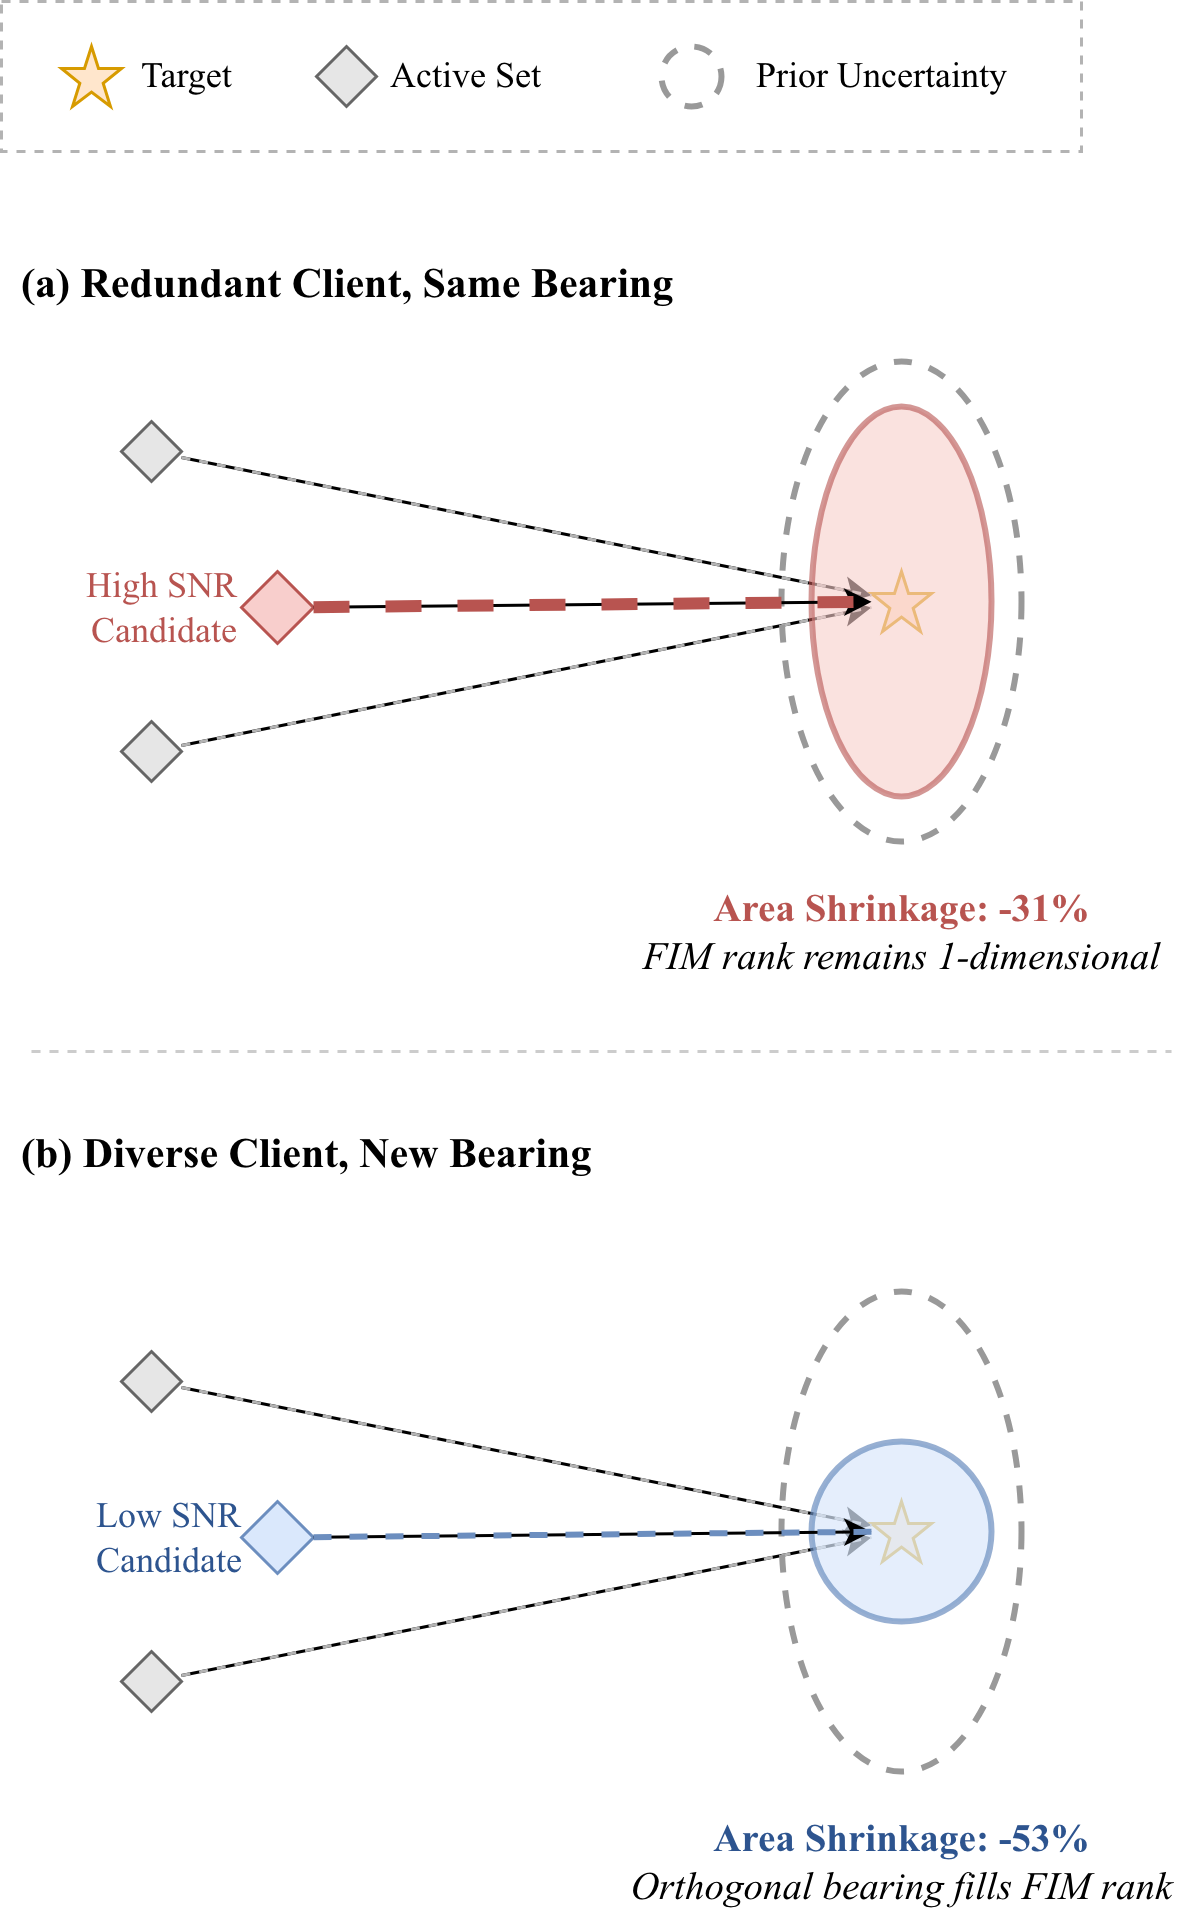
\includegraphics[width=\columnwidth]{fig_2.png}
\caption{Effect of angular diversity versus received signal strength on the target uncertainty ellipse. Two clients are already in the active set at the same bearing to the target, so the uncertainty ellipse is elongated and the aggregate FIM is effectively rank-one. \textbf{(a)} Adding a redundant client from the same bearing, even at high SNR, sharpens only the well-estimated axis; the uncertainty area shrinks by $31\%$ and the FIM remains effectively one-dimensional. \textbf{(b)} Adding a diverse client from an orthogonal bearing, even at low SNR, populates the deficient FIM direction and reduces the ellipse toward a circle, a $53\%$ reduction. Ellipses are computed from the FIM model of~\eqref{eq:fim}.}
\label{fig:geometry}
\end{figure}

Fig.~\ref{fig:geometry} illustrates this property. A redundant high-SNR addition from an occupied bearing shrinks the target uncertainty ellipse by $31\%$, whereas a diverse low-SNR addition from a new bearing shrinks it by $53\%$.

% ============================================================= III. PROBLEM FORMULATION
\section{Problem Formulation}\label{sec:formulation}
We now state the per-round selection problem. The \emph{learning utility} rewards a representative, diverse active set rather than the clients with the largest gradient magnitudes. Following the facility-location construction of DivFL~\cite{balakrishnan2022divfl}, each client is probed on the current global model to obtain a gradient embedding $\bg_k$, the nonnegative similarity is defined as
\begin{equation}
s(j,k)=\exp\!\Big(-\tfrac{\lVert \bg_j-\bg_k\rVert^{2}}{2\varsigma^{2}}\Big),
\label{eq:sim}
\end{equation}
with bandwidth $\varsigma$ set by the median heuristic, and a set is scored by how well its members cover the client population in gradient space,
\begin{equation}
U_{\mathrm{learn}}(\calS)=\sum_{j\in\calN}\max_{k\in\calS} s(j,k).
\label{eq:ulearn}
\end{equation}
The \emph{sensing utility} is the aggregate log-determinant of the FIM,
\begin{equation}
U_{\mathrm{sense}}(\calS)=\sum_{m=1}^{M}\logdet\!\big(\bJ_m(\calS)\big).
\label{eq:usense}
\end{equation}
The log-determinant is an appropriate information measure because it rewards populating directions of the FIM that are currently weak, which is precisely the angular-diversity behaviour of Fig.~\ref{fig:geometry}. Both~\eqref{eq:ulearn} and~\eqref{eq:usense} are monotone submodular. The composite utility is the nonnegative weighted sum
\begin{equation}
U(\calS)=\alpha\,U_{\mathrm{learn}}(\calS)+\lambda\,U_{\mathrm{sense}}(\calS)
+U_{\mathrm{aux}}(\calS),
\label{eq:composite}
\end{equation}
where the weight $\lambda\ge 0$ sets the learning--sensing trade-off and $U_{\mathrm{aux}}$ collects auxiliary coverage and fairness terms, which are also monotone submodular and carry fixed small weights as specified in Table~\ref{tab:setup}. In each round the scheduler solves
\begin{equation}
\begin{aligned}
\max_{\calS\subseteq\calN}\quad & U(\calS)\\
\text{s.t.}\quad & |\calS|=K,\qquad \mathrm{MSE}(\calS)\le\varepsilon .
\end{aligned}
\label{eq:problem}
\end{equation}
Problem~\eqref{eq:problem} is a cardinality-constrained submodular maximisation with an additional aggregation-MSE constraint. Even without the MSE constraint the problem is NP-hard~\cite{nemhauser1978}. We therefore do not seek the exact optimum, but rather a selection rule with a provable approximation guarantee and a principled mechanism for respecting the budget.

\begin{remark}[Scope of the baseline comparison]
A method that omits the $\lambda\,U_{\mathrm{sense}}$ term and the MSE constraint is free to maximise $U_{\mathrm{learn}}$ alone and will often attain higher accuracy precisely because it allocates no selection budget to sensing. A comparison against such methods does not measure the quality of the accuracy--sensing trade-off. The evaluation in Section~\ref{sec:results} is therefore restricted to methods that carry an explicit sensing objective.
\end{remark}

% ============================================================= IV. ALGORITHM
\section{The SCOUT-FL Algorithm}\label{sec:algorithm}
\scout{} solves~\eqref{eq:problem} with a greedy inner loop and a primal--dual outer loop. The design rests on two properties. First, the composite utility is monotone submodular, so greedy addition is near-optimal. Second, the aggregation-MSE budget is handled by a dual price on violation rather than a hard gate, so a temporarily tight budget adjusts the selection rather than eliminating candidate sets.

\subsection{Lagrangian Relaxation and Greedy Inner Selection}
The aggregation-MSE constraint is relaxed with a nonnegative dual variable $\mu\ge 0$, yielding the per-round Lagrangian utility
\begin{equation}
U_{\mu}(\calS)=U(\calS)-\mu\big(\mathrm{MSE}(\calS)-\varepsilon\big).
\label{eq:lagrangian}
\end{equation}
For a fixed $\mu$, the active set is grown greedily by adding the client with the largest marginal gain until $K$ clients are chosen,
\begin{equation}
k^\star=\arg\max_{k\notin\calS}\;\Big[U_{\mu}(\calS\cup\{k\})-U_{\mu}(\calS)\Big].
\label{eq:greedy}
\end{equation}
The marginal gain of the sensing term admits the closed form
\begin{equation}
\Delta_m(k\mid\calS)=\logdet\!\big(\bJ_m(\calS)+\bJ_{k,m}\big)-\logdet\!\big(\bJ_m(\calS)\big),
\end{equation}
which, via the matrix determinant lemma, is computed in $O(1)$ per target from the running inverse $\bJ_m(\calS)^{-1}$. No matrix is refactorised inside the loop, and lazy evaluation~\cite{krause2014submodular} avoids most re-scorings. A candidate whose marginal score is non-finite, corresponding to a degenerate geometry, is excluded from the maximisation.

\subsection{Primal--Dual Outer Update}
After the active set $\calS_t$ is realised and its aggregation MSE $\mathrm{MSE}(\calS_t)$ is measured, the dual variable ascends on the violation,
\begin{equation}
\mu_{t+1}=\big[\mu_t+\eta\,\big(\mathrm{MSE}(\calS_t)-\varepsilon\big)\big]_+,
\label{eq:dual}
\end{equation}
with step size $\eta>0$ and $[\cdot]_+=\max(\cdot,0)$. In implementation the violation is expressed relative to the budget as $\mathrm{MSE}(\calS_t)/\varepsilon-1$, so the step $\eta$ acts on a dimensionless quantity and needs no retuning across budget scales. At slack operating points the two forms coincide, since $\mu$ remains at zero under both. The update is self-correcting. Rounds that exceed the budget raise $\mu$, which increases the penalty on high-MSE clients in the next round's greedy step, whereas rounds that remain under budget relax $\mu$ toward zero, allowing the scheduler to allocate its budget to learning and sensing. The update also completes the cognitive cycle of the scheduler. The greedy step is the decision, the joint transmission is the action, the measured aggregation error is the observation, and the dual ascent is the learning step that conditions the next decision on the observed outcome. Algorithm~\ref{alg:scout} summarises the procedure.

\begin{algorithm}[t]
\caption{\scout{}: sensing-aware primal--dual selection}
\label{alg:scout}
\begin{algorithmic}[1]
\STATE \textbf{Input:} clients $\calN$, budget $K$, tolerance $\varepsilon$, weight $\lambda$, dual step $\eta$
\STATE Initialise $\bw_0$, dual $\mu_0\gets 0$
\FOR{round $t=0,1,\dots,T-1$}
  \STATE probe clients: gradient embeddings $\{\bg_{k}\}$, channels $\{h_{k,t}\}$, geometry $\{\bJ_{k,m}\}$
  \STATE $\calS_t\gets\emptyset$; initialise running inverses $\bJ_m(\emptyset)^{-1}$
  \FOR{$i=1$ to $K$}
     \STATE $k^\star\gets\arg\max_{k\notin\calS_t}\, U_{\mu_t}(\calS_t\cup\{k\})-U_{\mu_t}(\calS_t)$
     \STATE $\calS_t\gets\calS_t\cup\{k^\star\}$; rank-two update of each $\bJ_m^{-1}$
  \ENDFOR
  \STATE broadcast $\bw_t$; clients in $\calS_t$ run local SGD
  \STATE aggregate over the air via~\eqref{eq:aircomp}; measure $\mathrm{MSE}(\calS_t)$
  \STATE $\bw_{t+1}\gets$ AirComp aggregate of $\{\Delta\bw_{k,t}\}$
  \STATE $\mu_{t+1}\gets[\mu_t+\eta(\mathrm{MSE}(\calS_t)-\varepsilon)]_+$
\ENDFOR
\STATE \textbf{return} $\bw_T$
\end{algorithmic}
\end{algorithm}

\begin{remark}[Hard-gate ablation, \scout{}$^{\dagger}$]
Replacing the dual penalty in~\eqref{eq:lagrangian} with a hard feasibility filter, i.e.\ greedily selecting only among clients that keep $\mathrm{MSE}(\calS)\le\varepsilon$, yields the ablation \scout{}$^{\dagger}$. It employs the same selection machinery without the soft, self-tuning budget and serves to isolate the contribution of the primal--dual mechanism.
\end{remark}

% ============================================================= V. THEORY
\section{Theoretical Analysis}\label{sec:theory}
This section establishes four results. First, the composite utility is monotone submodular, so greedy selection is near-optimal, and a curvature refinement sharpens the approximation constant. Second, the primal--dual loop is asymptotically feasible with vanishing regret. Third, the CRB optimised by the algorithm is an achievable performance measure. Fourth, the aggregation-error budget enters an explicit convergence bound on the learning iterate, which closes the loop between the constraint that the cognitive scheduler enforces and the model that the network trains. The scope of the greedy guarantee is stated precisely. Proofs are given in the Appendix.

\begin{proposition}[Monotone submodularity of the utility]\label{prop:submod}
The learning utility~\eqref{eq:ulearn} is a facility-location function with nonnegative similarities and is therefore monotone submodular~\cite{balakrishnan2022divfl,krause2014submodular}. For each target $m$, the map $\calS\mapsto\logdet(\bJ_m(\calS))$ with $\bJ_m(\calS)=\bJ_0+\sum_{k\in\calS}\bJ_{k,m}$, $\bJ_0\succ 0$, $\bJ_{k,m}\succeq 0$, is monotone non-decreasing and submodular. Consequently the composite $U$ in~\eqref{eq:composite}, a nonnegative weighted sum of monotone submodular terms, is monotone submodular.
\end{proposition}

\begin{proposition}[Greedy guarantee for the utility]\label{prop:greedy}
Let $U^\star$ be the maximum of $U$ over sets of size $K$. The greedy rule~\eqref{eq:greedy} applied to $U$ (i.e.\ at $\mu=0$) returns a set $\calS^{\mathrm{g}}$ with $U(\calS^{\mathrm{g}})\ge(1-1/e)\,U^\star$.
\end{proposition}

\begin{remark}[Curvature-sharpened guarantee]\label{rem:curvature}
The constant in Proposition~\ref{prop:greedy} improves when the utility is not fully curved. Let the total curvature of $U$ be
$\gamma_U=1-\min_{k\in\calN}\big[U(\calN)-U(\calN\setminus\{k\})\big]/U(\{k\})\in[0,1]$.
Greedy selection under a cardinality constraint then attains the factor $\frac{1}{\gamma_U}\big(1-e^{-\gamma_U}\big)$, which is at least $1-1/e$ and strictly exceeds it whenever $\gamma_U<1$~\cite{conforti1984}. Both components of $U$ satisfy $\gamma_U<1$ in this system. The prior $\bJ_0\succ 0$ keeps every sensing marginal strictly positive even on the full ground set, and the facility-location term retains positive marginals whenever some client remains the best cover for at least one peer. At the operating point of Section~\ref{sec:results} the prior is deliberately weak ($\lambda_0=10^{-3}$), so the measured curvature of the sensing utility is close to one ($\gamma\approx 0.999$ across the campaign scenarios) and the sharpened factor exceeds the classical constant only marginally ($0.6323$ against $0.6321$). The refinement is stated for completeness. It becomes material when the prior carries substantial target information, for example when knowledge accumulates across rounds.
\end{remark}

Proposition~\ref{prop:greedy} applies to $U$, whereas the inner loop of Algorithm~\ref{alg:scout} optimises the penalised objective $U_\mu$. The following proposition delineates the guarantee that holds in each regime.

\begin{proposition}[Guarantees for the penalised objective]\label{prop:penalised}
Write $U_\mu=U-\mu(\mathrm{MSE}-\varepsilon)$. \emph{(i)} When the constraint is slack, as at the main operating point of Section~\ref{sec:results} (realised aggregation MSE $2\times10^{-4}$ against a budget $\varepsilon=10^{-3}$), the dual variable satisfies $\mu=0$, hence $U_\mu=U$ and the $(1-1/e)$ bound of Proposition~\ref{prop:greedy} applies exactly. \emph{(ii)} For $\mu>0$, the penalty $-\mu\,\mathrm{MSE}(\calS)$ is, under the channel-inversion model~\eqref{eq:mse}, a min-based set-coupled term that is neither modular nor submodular; hence $U_\mu$ is not guaranteed submodular and the $(1-1/e)$ bound does not transfer to $U_\mu$. In this regime feasibility is delivered by the outer dual update~\eqref{eq:dual}, a separate no-regret mechanism analysed in Proposition~\ref{prop:pd}, while the greedy inner step, which excludes non-positive marginals, keeps the selection within the monotone-improvement region. No constant-factor guarantee is claimed for $U_\mu$ in the binding regime; deterministic greedy selection admits no such guarantee for non-monotone submodular objectives, for which the relevant bound is the $1/e$ factor of randomised greedy~\cite{buchbinder2014}.
\end{proposition}

\begin{proposition}[Feasibility and regret of the primal--dual loop]\label{prop:pd}
Suppose $\mathrm{MSE}(\calS_t)\in[0,G]$ for all $t$ and let $\eta=\Theta(1/\sqrt{T})$. Then the time-averaged constraint violation vanishes, $\frac{1}{T}\sum_{t}(\mathrm{MSE}(\calS_t)-\varepsilon)\le O(1/\sqrt{T})$, and the cumulative utility gap to the best fixed feasible selection in hindsight is $O(\sqrt{T})$; the loop is no-regret.
\end{proposition}

\begin{proposition}[CRB achievability]\label{prop:crb}
Under the asymptotic-normality regime of Section~\ref{sec:sensing}, the maximum-likelihood (ML) position estimator is efficient, and its error covariance approaches $\bJ_m(\calS)^{-1}$, so the CRB in~\eqref{eq:crb} is attained. Differences in CRB between active sets therefore correspond to differences in achievable localisation error rather than differences in a loose bound.
\end{proposition}

Proposition~\ref{prop:crb} establishes that the accuracy--CRB frontier represents a genuine performance trade-off. Section~\ref{sec:results} confirms this empirically (Fig.~\ref{fig:rmse}).

The final result connects the aggregation budget to the learning iterate. It rests on three standard assumptions. \emph{(A1)} The global objective $F$ is $L$-smooth and bounded below by $F^\star$. \emph{(A2)} The aggregated update is an unbiased estimate of the negative scaled gradient, $\mathbb{E}[\sum_k p_{k,t}\Delta\bw_{k,t}\,|\,\bw_t]=-\eta_\ell\nabla F(\bw_t)$ with $\eta_\ell>0$, and its variance about that mean is at most $\eta_\ell^2\sigma_u^2$. \emph{(A3)} The AirComp receiver noise contributes a per-round aggregation MSE of $\mathrm{MSE}(\calS_t)$, as defined in~\eqref{eq:mse}. Assumption (A2) abstracts the selection bias of a deterministic scheduler. The facility-location term steers every active set toward a representative cover of the client population, which keeps the aggregated update close to its population mean, and the bound should be read under that qualification.

\begin{proposition}[Learning convergence under the aggregation budget]\label{prop:learn}
Under (A1)--(A3) and any $\eta_\ell\le 1/L$, the iterates of Algorithm~\ref{alg:scout} satisfy
\begin{equation}
\frac{1}{T}\sum_{t=1}^{T}\mathbb{E}\big\lVert\nabla F(\bw_t)\big\rVert^{2}
\le\frac{2\big(F(\bw_1)-F^\star\big)}{\eta_\ell T}
+L\eta_\ell\Big(\sigma_u^{2}+\frac{\overline{\mathrm{MSE}}_T}{\eta_\ell^{2}}\Big),
\label{eq:learnbound}
\end{equation}
where $\overline{\mathrm{MSE}}_T=\frac{1}{T}\sum_t\mathrm{MSE}(\calS_t)$. By Proposition~\ref{prop:pd} the dual loop guarantees $\overline{\mathrm{MSE}}_T\le\varepsilon+O(1/\sqrt{T})$, so the bound converges to a noise floor that scales linearly in the prescribed budget $\varepsilon$. With a diminishing local scale $\eta_\ell=\Theta(1/\sqrt{T})$ the average squared gradient norm is $O\big((1+\sigma_u^{2})/\sqrt{T}+\sqrt{T}\,\varepsilon\big)$, which for a budget $\varepsilon=O(1/T)$ recovers the standard $O(1/\sqrt{T})$ rate of noiseless federated SGD.
\end{proposition}

Proposition~\ref{prop:learn} is the quantitative payoff of the cognitive loop. The scheduler does not merely respect an operational constraint. Through~\eqref{eq:learnbound} the constraint level $\varepsilon$ becomes a design parameter with a provable effect on the trained model, and the dual price is the mechanism that delivers the required time-averaged error without manual tuning. At the main operating point the budget is slack by an order of magnitude, so the noise floor in~\eqref{eq:learnbound} is dominated by the sampling variance $\sigma_u^2$.

% ============================================================= VI. RESULTS
\section{Numerical Results}\label{sec:results}

\subsection{Experimental Setup}
The ISAC-FL network is simulated with $N=100$ clients, a per-round budget of $K=10$, and $T=150$ rounds. The learning task at the main operating point is CIFAR-10 image classification with a compact convolutional neural network (CNN), split across clients by a Dirichlet partition. Cross-dataset results additionally cover CIFAR-100, EMNIST, Fashion-MNIST, and UCI-HAR (real datasets, loaded through \texttt{torchvision}). The wireless model uses Rayleigh and Rician fading with a physical link budget, AirComp with channel-inversion precoding, and an aggregation-MSE tolerance $\varepsilon$. The sensing scene contains $M$ targets with configurable angular spread. Robustness is assessed through a one-factor-at-a-time (OFAT) campaign that sweeps data partition and heterogeneity, channel model and SNR, and target count and angular spread; every configuration is repeated over $5$ random seeds. Table~\ref{tab:setup} lists the parameters. All results compare \scout{} against sensing-aware baselines only.

\begin{table}[!t]
\centering
\caption{Experimental configuration.}
\label{tab:setup}
\renewcommand{\arraystretch}{1.15}
\resizebox{\columnwidth}{!}{%
\begin{tabular}{@{}ll@{}}
\toprule
Parameter & Value \\
\midrule
Clients $N$ / budget $K$ / rounds $T$ & $100$ / $10$ / $150$ \\
Seeds per configuration & $5$ \\
Main task / model & CIFAR-10 / compact CNN \\
Cross-dataset tasks & CIFAR-100, EMNIST, F-MNIST, UCI-HAR \\
Data partition / heterogeneity & Dirichlet, $\alpha\in\{0.1,0.3,0.5\}$ (nom.\ $0.3$) \\
Local SGD & learning rate $0.05$, momentum $0.9$ \\
 & $1$ local epoch, batch size $64$ \\
Train / test subsample & $20{,}000$ / $4{,}000$ \\
Channel / carrier & Rayleigh, Rician ($K{=}6$ dB) / $3.5$ GHz \\
Tx power / noise figure & $-15$ dBm / $7$ dB \\
Receive SNR sweep & $0$ down to $-35$ dB \\
Targets $M$ / angular spread $\kappa_a$ & $\{2,3,5\}$ / $\{0.02,0.05,0.1\}$ \\
FIM constants $\kappa_r,\kappa_a,\lambda_0$ & $1.0,\ 0.05,\ 10^{-3}$ \\
Utility weights $\alpha,\lambda,\lambda_{\mathrm{cov}},\lambda_{\mathrm{fair}}$ & $1.0,\ 1.0,\ 0.5,\ 0.3$ \\
Aggregation-MSE budget $\varepsilon$ / dual step $\eta$ & $10^{-3}$ / $0.5$ \\
\bottomrule
\end{tabular}}
\end{table}

\subsubsection*{Remarks on absolute accuracy}
The absolute accuracy is set by the deliberately constrained federated regime, namely a compact CNN, a $20{,}000$-image subsample over $100$ clients, $10\%$ participation, non-IID data, and AirComp noise in every round. Training has converged at $T=150$, since the curves vary by less than $0.1$ percentage points over the final $25$ rounds, and controlled runs verified that a larger network does not raise the plateau under the aggregation noise. The quantity of interest in a client-selection study is the relative gap between selectors at a fixed, converged operating point. Both final and peak accuracy are reported for every method.

\subsection{Baselines}
The comparison set contains eleven sensing-aware methods. Methods that correspond to published schemes are cited; methods marked as reconstructions implement a stated design principle and do not correspond to a single published algorithm.
\begin{itemize}
\item \textbf{Asaad}~\cite{asaad2025}, the state-of-the-art reference, performs sensing-aware device pruning under a combined aggregation-MSE and CRB metric.
\item \textbf{OTA-FL-ISCC}~\cite{zheng2024otafliscc}, \textbf{Fed-ISCC}~\cite{du2024fediscc}, and \textbf{ISCC-Air-FEEL}~\cite{wen2025isccairfeel} are published ISAC-FL schemes. ISCC-Air-FEEL is applied as the selection restriction of its resource-allocation objective, since device scheduling is deferred to future work in the original.
\item \textbf{CRB-Only} and \textbf{Sensing-Only} are the classical A-optimal (trace of the inverse FIM) and D-optimal (log-determinant of the FIM) design criteria~\cite{kay1993,krause2014submodular}, respectively.
\item \textbf{CollabSenseFed}, \textbf{Sensing-Native}, \textbf{Fixed-Weighted}, \textbf{FedAvg-ISCC}, and \textbf{FedSGD-ISCC} are reconstructions of common design principles, namely equal-weight learning-plus-sensing selection, gradient-reuse sensing, a hand-set weighted sum, and throughput-based ISCC selection differing only in the local-update rule.
\end{itemize}
The hard-gate ablation \scout{}$^{\dagger}$ is also reported.

\subsection{The Learning--Sensing Frontier}
Fig.~\ref{fig:frontier} presents the principal result. Each marker places a method by its final accuracy and final-round CRB at the main operating point, with higher accuracy and lower CRB being preferable. \scout{} attains the highest accuracy among all methods inside the sensing-competitive band. Methods that reach comparable accuracy do so only at substantially larger CRB; in particular, OTA-FL-ISCC matches the accuracy of \scout{} but exits the sensing-competitive band entirely. Conversely, the methods that achieve the lowest CRB (Asaad, CRB-Only) incur an accuracy reduction of eight to nine percentage points. \scout{} does not attain the minimum CRB; it attains the maximum accuracy among the methods that remain within the sensing-competitive region.

\begin{figure}[!t]
\centering
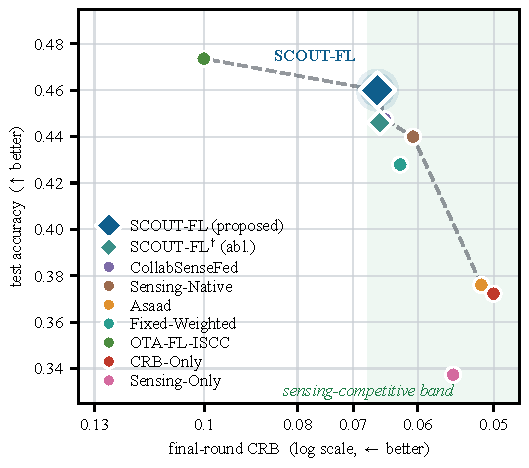
\includegraphics[width=\columnwidth]{fig3_frontier.pdf}
\caption{Learning--sensing frontier at the main operating point (final-round CRB, logarithmic axis; $5$ seeds). \scout{} attains the highest accuracy inside the sensing-competitive band. Four ISAC baselines with $\mathrm{CRB}>0.4$ are dominated on both axes and omitted for scale. The dashed line is the Pareto frontier over the sensing-aware pool.}
\label{fig:frontier}
\end{figure}

Table~\ref{tab:main} quantifies the frontier and reports final and peak accuracy side by side. \scout{} reaches $46.0\%$ final accuracy ($48.8\%$ peak), ahead of every sensing-aware competitor on both measures, at a final-round CRB of $0.066$, which is within approximately $9\%$ of the best-sensing method's CRB while carrying $8$--$12$ percentage points more accuracy than the low-CRB methods. Its realised aggregation MSE of $2.0\times10^{-4}$ is an order of magnitude below the budget, so the primal--dual constraint is slack at this operating point; Section~\ref{sec:threshold} examines the effect of tightening the sensing requirement. The frontier position is also weight-free. Defining a method as Pareto-optimal at an operating point when no sensing-aware method exceeds it on both accuracy and CRB simultaneously, \scout{} is non-dominated in $96\%$ of operating points under each CRB convention (Fig.~\ref{fig:gapdist}; the single dominated point is the strongly non-IID partition $\alpha=0.1$, where Sensing-Native prevails), a statement that requires no choice of weighting between the two axes.

Fig.~\ref{fig:gapdist} widens the view to the full campaign, measuring every method's final accuracy against the best sensing-aware method at each of the $25$ operating points. \scout{} combines the smallest accuracy gaps of any method that retains a high Pareto share (median $1.3$ percentage points, never exceeding $4.7$) with non-dominance at $96\%$ of the points. The only method with smaller gaps, OTA-FL-ISCC, attains them by abandoning the sensing objective, which Fig.~\ref{fig:frontier} shows places it outside the sensing-competitive band, while the methods with comparable sensing investment (Asaad, CRB-Only, Sensing-Only) sit $8$--$13$ percentage points behind the field.

\begin{figure}[!t]
\centering
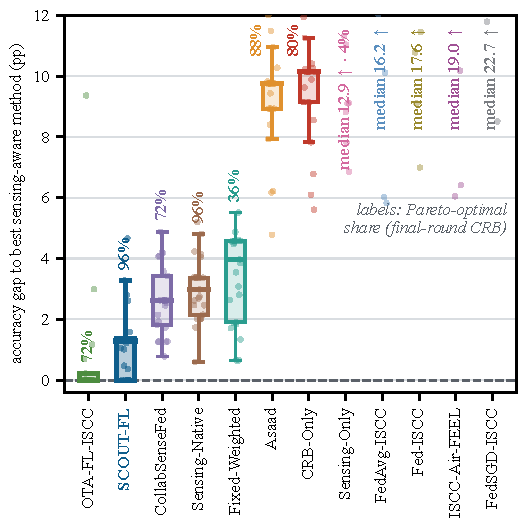
\includegraphics[width=\columnwidth]{fig_gap_dist.pdf}
\caption{Accuracy gap to the best sensing-aware method at each of the $25$ operating points ($5$ seeds, seed-averaged, so the best method at a point has zero gap). Boxes span the IQR with $1.5\times$IQR whiskers, dots are operating points, methods are ordered by median gap, and the median is printed for the five off-scale methods. Percentages give each method's Pareto-optimal share under the final-round CRB convention. Under the round-mean convention the shares agree within $\pm16$~pp and are identical ($96\%$, $24/25$) for \scout{}. Methods at $0\%$ carry no label.}
\label{fig:gapdist}
\end{figure}

\begin{table}[!t]
\centering
\caption{Main operating point (CIFAR-10, $5$ seeds). Accuracy as final\,$\pm$\,std and peak; CRB in both conventions; aggregation MSE. Sensing-aware pool only. Best in \textbf{bold}.}
\label{tab:main}
\renewcommand{\arraystretch}{1.2}
\setlength{\tabcolsep}{3.5pt}
\resizebox{\columnwidth}{!}{%
\begin{tabular}{@{}lccccc@{}}
\toprule
Method & Acc.\ final & Acc.\ peak & CRB$_{\text{fin}}$ & CRB$_{\text{mean}}$ & MSE \\
\midrule
\textbf{\scout{}}          & \textbf{46.0}\,$\pm$\,2.3 & \textbf{48.8} & 0.066 & 0.067 & $2.0e{-}4$ \\
\scout{}$^{\dagger}$ (abl.)  & 44.6\,$\pm$\,2.0 & 48.0 & 0.066 & 0.066 & $2.0e{-}4$ \\
CollabSenseFed             & 44.7\,$\pm$\,1.9 & 47.0 & 0.065 & 0.062 & $2.0e{-}4$ \\
Sensing-Native             & 44.0\,$\pm$\,2.0 & 46.7 & 0.061 & 0.062 & $2.0e{-}4$ \\
Fixed-Weighted             & 42.8\,$\pm$\,1.9 & 47.2 & 0.063 & 0.065 & $2.0e{-}4$ \\
Asaad~\cite{asaad2025}     & 37.6\,$\pm$\,3.3 & 39.4 & \textbf{0.052} & \textbf{0.052} & $1.5e{-}4$ \\
CRB-Only                   & 37.2\,$\pm$\,3.1 & 39.2 & 0.050 & 0.050 & $1.8e{-}4$ \\
Sensing-Only               & 33.7\,$\pm$\,7.3 & 36.5 & 0.055 & 0.055 & $1.9e{-}4$ \\
\bottomrule
\end{tabular}}
\end{table}

\subsection{Paired Comparison Against the Strongest Baselines}
Fig.~\ref{fig:gapdist} summarises the field-wide gap distribution; Fig.~\ref{fig:paired} complements it by resolving the per-point uncertainty against the two strongest rivals, pairing \scout{} against each of them point-by-point across the campaign with $95\%$ confidence intervals. The accuracy gains are consistent across operating points. Aggregated over the campaign (Table~\ref{tab:h2h}), \scout{} improves final accuracy by $1.4$ percentage points over CollabSenseFed, $1.8$ over Sensing-Native, and $8.2$ over the state-of-the-art Asaad reference, while the CRB differences are small and of mixed sign, consistent with the intended frontier trade-off. Because the OFAT operating points share a common nominal configuration and are therefore not statistically independent, the Wilcoxon signed-rank statistics are reported as descriptive summaries over a correlated sweep; the per-seed dispersion within each point (Table~\ref{tab:main}) provides the complementary measure over independent replicates.

\begin{figure}[!t]
\centering
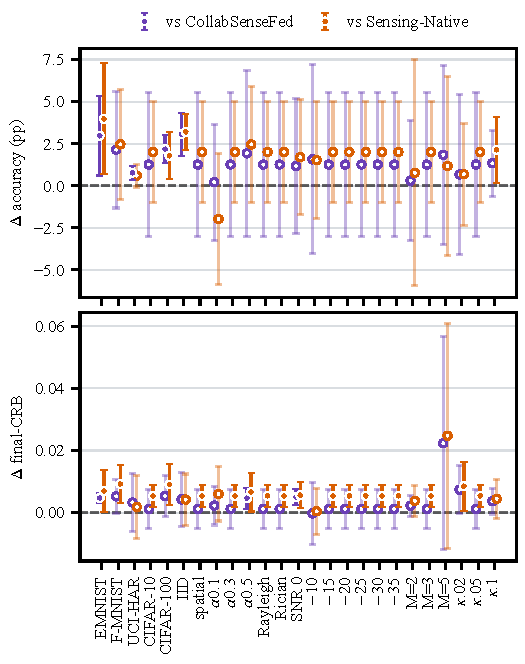
\includegraphics[width=\columnwidth]{fig4_paired_delta.pdf}
\caption{Paired per-operating-point differences of \scout{} versus the two strongest sensing-aware baselines, with $95\%$ bootstrap confidence intervals. Hollow markers denote points whose interval crosses zero. Accuracy differences (top) are consistently positive; CRB differences (bottom) are small.}
\label{fig:paired}
\end{figure}

\begin{table}[!t]
\centering
\caption{Paired comparison over the campaign (per-point mean difference, \scout{} minus baseline). Positive $\Delta$Acc favours \scout{}. The dependence structure of the operating points is discussed in the text.}
\label{tab:h2h}
\renewcommand{\arraystretch}{1.2}
\begin{tabular}{@{}lccc@{}}
\toprule
Baseline & $\Delta$Acc (pp) & $\Delta$CRB$_{\text{fin}}$ & Wilcoxon $p$ \\
\midrule
CollabSenseFed & $+1.4$ & $+0.003$ & $<10^{-3}$ \\
Sensing-Native & $+1.8$ & $+0.006$ & $<10^{-3}$ \\
Asaad~\cite{asaad2025} & $+8.2$ & $+0.015$ & $<10^{-3}$ \\
\bottomrule
\end{tabular}
\end{table}


\subsection{Selection of the Trade-Off Weight $\lambda$}\label{sec:lambda}
The weight $\lambda$ in~\eqref{eq:composite} is the sole parameter that positions \scout{} on the frontier, and it is swept explicitly. Fig.~\ref{fig:lambda} traces the accuracy and CRB of \scout{} as $\lambda$ ranges from $0$ (learning only) upward. As $\lambda$ grows, the selection allocates more of its budget to angular diversity, the CRB decreases, and the accuracy declines gradually, tracing the accuracy--CRB frontier. The operating-point value $\lambda=1$, at which the normalised learning and sensing utilities contribute comparably, lies at the accuracy-favouring knee of this curve; beyond it, additional sensing weight reduces accuracy faster than it improves the CRB. The value $\lambda=1$ is used throughout, and nearby values shift the operating point only gradually.

\begin{figure}[!t]
\centering
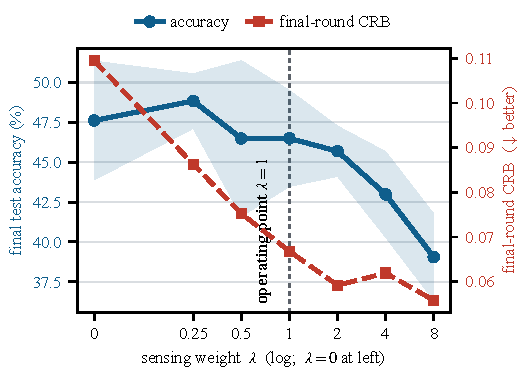
\includegraphics[width=\columnwidth]{fig9_lambda.pdf}
\caption{Effect of the trade-off weight $\lambda$ (\scout{}, main operating point, $5$ seeds). As $\lambda$ increases, accuracy (left axis) declines gradually while the CRB (right axis) decreases, tracing the accuracy--CRB frontier. The operating point $\lambda=1$ lies at the accuracy-favouring knee.}
\label{fig:lambda}
\end{figure}

\subsection{Convergence}
Fig.~\ref{fig:convergence} tracks accuracy and sensing information over the $150$ rounds for all twelve sensing-aware methods. \scout{} reaches the highest accuracy level and maintains it, while its sensing log-determinant remains in the middle of the field, reflecting the design decision to expend part of the sensing headroom on accuracy. The round-by-round view also exposes the Pareto structure. The baselines that reach the late-round accuracy of \scout{} are precisely those at the bottom of the sensing panel, i.e.\ those that have ceased to invest in sensing. The accuracy curves are flat beyond round $125$, confirming convergence.

\begin{figure}[!t]
\centering
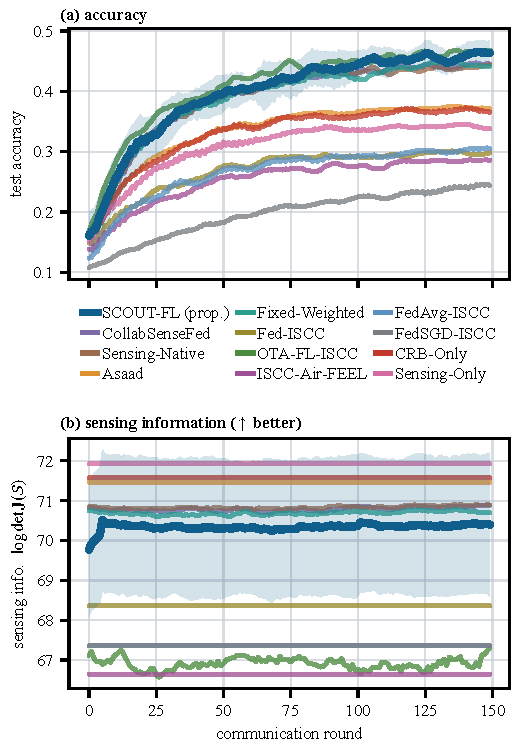
\includegraphics[width=\columnwidth]{fig7_convergence.pdf}
\caption{Per-round accuracy (top) and sensing log-determinant (bottom, higher is better) for all twelve sensing-aware methods; \scout{} in bold with $\pm$std band. \scout{} leads on accuracy while holding a mid-field sensing level; methods that match its accuracy occupy the bottom of the sensing panel.}
\label{fig:convergence}
\end{figure}

\subsection{Sensitivity to the Sensing Requirement}\label{sec:threshold}
The dependence of the method ranking on the stringency of the sensing requirement is relevant for deployment. Fig.~\ref{fig:threshold} counts, for each sensing threshold $\mathrm{CRB}\le\tau$, how often each method is the most accurate selection that still meets the threshold. At tight thresholds the sensing-heavy methods prevail, because only they qualify. Across the operationally relevant band $\tau\in[0.07,0.13]$, \scout{} wins the constrained-accuracy comparison at nearly every point. Only at very loose thresholds do methods without effective sensing investment re-enter. This behaviour reflects the function of the primal--dual budget, which places \scout{} at the accuracy-favouring end of the feasible region whenever sensing is required but not extreme.

\begin{figure}[!t]
\centering
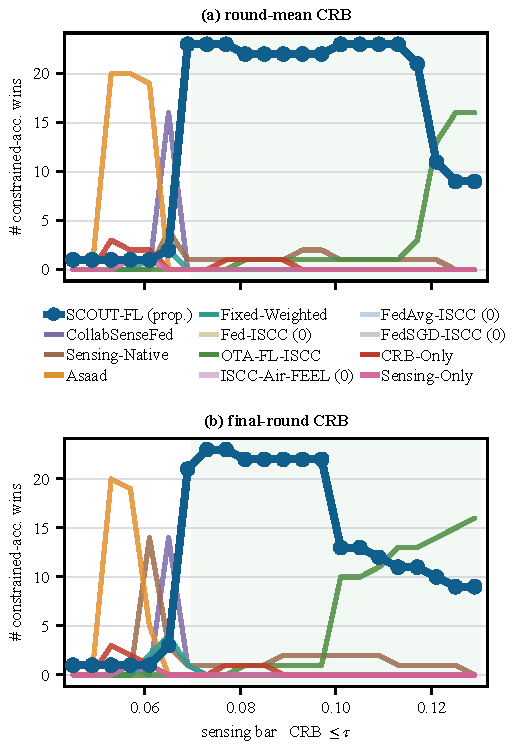
\includegraphics[width=\columnwidth]{fig6_threshold.pdf}
\caption{Constrained-accuracy wins versus the sensing threshold $\tau$, under both CRB conventions, for every sensing-aware competitor (methods with zero wins marked ``$(0)$''). \scout{} wins across the operational band; the tightest thresholds favour the sensing-heavy methods.}
\label{fig:threshold}
\end{figure}

\subsection{Cross-Dataset Generalisation}
Table~\ref{tab:cross} repeats the comparison on five datasets, reporting final and peak accuracy. Among the sensing-competitive methods, \scout{} attains the highest accuracy on every dataset by both measures, and its CRB remains within a competitive band of the sensing-heavy baselines throughout. The sensing utility is decoupled from the learning task by construction, since the FIM in (4) and (5) depends only on the physical geometry of the active set and never on the gradient embeddings of (9). Accordingly, the absolute accuracy scales with dataset complexity while the relative margin of \scout{} and its CRB level are preserved across all five datasets. The advantage is therefore not specific to a particular dataset.

\begin{table}[!t]
\centering
\caption{Cross-dataset accuracy as final\,(peak) \% and final-round CRB (mean over $5$ seeds). Best accuracy in \textbf{bold}.}
\label{tab:cross}
\renewcommand{\arraystretch}{1.2}
\setlength{\tabcolsep}{3pt}
\resizebox{\columnwidth}{!}{%
\begin{tabular}{@{}lccccc@{}}
\toprule
 & CIFAR-10 & CIFAR-100 & EMNIST & F-MNIST & UCI-HAR \\
\midrule
\multicolumn{6}{@{}l}{\emph{Accuracy, final (peak) \%}}\\
\textbf{\scout{}} & \textbf{46.0}\,(48.8) & \textbf{16.3}\,(16.6) & \textbf{72.0}\,(73.5) & \textbf{83.0}\,(84.1) & \textbf{92.5}\,(93.3) \\
CollabSenseFed & 44.7\,(47.0) & 14.1\,(15.0) & 69.0\,(70.8) & 80.8\,(83.5) & 91.7\,(92.8) \\
Sensing-Native & 44.0\,(46.7) & 14.5\,(15.1) & 68.0\,(70.2) & 80.5\,(83.4) & 91.8\,(93.0) \\
Asaad~\cite{asaad2025} & 37.6\,(39.4) & 10.5\,(11.6) & 60.0\,(61.9) & 78.2\,(79.6) & 83.0\,(84.0) \\
\midrule
\multicolumn{6}{@{}l}{\emph{Final-round CRB}}\\
\scout{} & 0.066 & 0.068 & 0.066 & 0.071 & 0.066 \\
CollabSenseFed & 0.065 & 0.062 & 0.062 & 0.066 & 0.062 \\
Sensing-Native & 0.061 & 0.058 & 0.059 & 0.062 & 0.064 \\
Asaad~\cite{asaad2025} & 0.052 & 0.052 & 0.052 & 0.052 & 0.052 \\
\bottomrule
\end{tabular}}
\end{table}

\subsection{Ablation and Selection Overhead}\label{sec:overhead}
Table~\ref{tab:ablation} isolates the effect of the soft constraint. Replacing the dual price with a hard feasibility gate (\scout{}$^{\dagger}$) reduces final accuracy by $1.4$ percentage points at the main operating point while leaving the CRB essentially unchanged, because the gate occasionally discards strong candidate sets that marginally exceed the budget. Section~\ref{sec:adapt} examines the binding regime and a mid-run budget change directly. Fig.~\ref{fig:runtime} reports the selection overhead, defined as the per-round wall-clock time of the selection step. The greedy loop of \scout{} with rank-two FIM updates requires approximately $36$~ms for $N=100$, $K=10$, comparable to the lightweight baselines and approximately one-seventh of the selection overhead of the state-of-the-art Asaad reference. The computational complexity of the sensing-driven selection is $O(KNM)$; the greedy loop performs $K$ additions, each scoring up to $N$ candidates, and each candidate's sensing marginal is evaluated in $O(1)$ per target across the $M$ targets through the closed-form rank-two update. The facility-location learning term contributes a further $O(KN^2)$ coverage update. Both terms are dominated by the gradient probe in practice, and the measured selection overhead grows near-linearly in $N$ and $K$.

\begin{table}[!t]
\centering
\caption{Constraint-handling ablation at the main operating point.}
\label{tab:ablation}
\renewcommand{\arraystretch}{1.2}
\setlength{\tabcolsep}{4pt}
\resizebox{\columnwidth}{!}{%
\begin{tabular}{@{}lccc@{}}
\toprule
Variant & Acc.\ final/peak (\%) & CRB$_{\text{fin}}$ & MSE \\
\midrule
\textbf{\scout{}} (primal--dual, soft) & \textbf{46.0}/\textbf{48.8} & 0.066 & $2.0e{-}4$ \\
\scout{}$^{\dagger}$ (hard gate)        & 44.6/48.0 & 0.066 & $2.0e{-}4$ \\
\bottomrule
\end{tabular}}
\end{table}

\begin{figure}[!t]
\centering
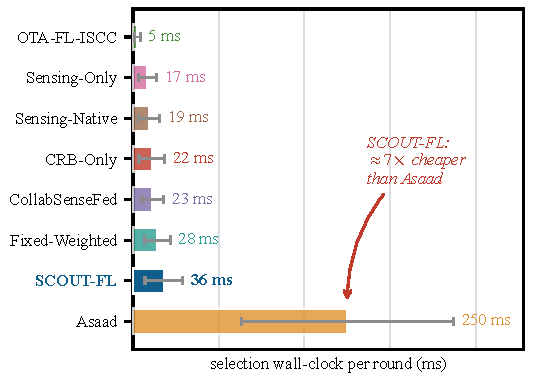
\includegraphics[width=\columnwidth]{fig10_runtime.pdf}
\caption{Selection overhead per round ($N=100$, $K=10$, mean\,$\pm$\,std over rounds and seeds). Greedy selection grows near-linearly in $N$ and needs about one-seventh of the overhead of the Asaad reference.}
\label{fig:runtime}
\end{figure}

\subsection{Adaptation Under a Budget Change}\label{sec:adapt}
The cognitive loop is exercised by cutting the aggregation budget at round $75$ from $\varepsilon=10^{-3}$ to $1.5\times10^{-4}$, below the realised error floor of $2.0\times10^{-4}$, so a constraint that was slack for the whole first half suddenly binds. Fig.~\ref{fig:adapt}(a) and (b) show the response over $5$ seeds. The dual price is zero before the cut, rises within one round of the first violation, and settles once the selection conforms. Every seed recovers a budget-feasible active set within two rounds. The time-averaged MSE after recovery is $1.51\times10^{-4}$ against a budget of $1.50\times10^{-4}$, with single rounds oscillating around the boundary. This is the time-average feasibility that Proposition~\ref{prop:pd} guarantees. Under the same disturbance the hard gate stays feasible in every round but finishes at $40.8\pm3.5\%$ accuracy against $42.3\pm3.8\%$ for the soft loop.

Fig.~\ref{fig:adapt}(c) and (d) sweep the static budget into the binding regime. The soft loop spends the whole budget, keeping the realised time-averaged MSE within one percent of $\varepsilon$ at every binding level, whereas the hard gate leaves ten to twenty percent unused because its per-client threshold must hold in every realisation. The unused budget costs the hard gate $4.6$ percentage points at the marginally binding level $\varepsilon=2\times10^{-4}$. Deep in the binding regime the two variants coincide within seed noise, and at the slack operating point they are indistinguishable, consistent with Table~\ref{tab:ablation}. The soft constraint therefore helps precisely where the budget is tight enough to matter but loose enough that discarding whole candidate sets wastes information.

\begin{figure}[!t]
\centering
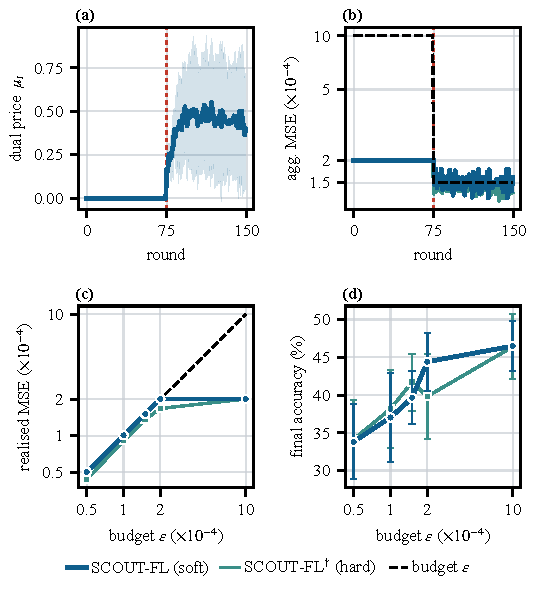
\includegraphics[width=\columnwidth]{fig12_adapt_sweep.pdf}
\caption{The primal--dual budget mechanism under stress ($5$ seeds). Top row, mid-run budget cut at round $75$: \textbf{(a)} the dual price is zero while the budget is slack and rises within one round of the first violation, and \textbf{(b)} the realised MSE returns to the new budget within two rounds and tracks it in time average. Bottom row, static budget sweep: \textbf{(c)} the soft loop follows the identity line to within one percent until the error floor is reached, while the hard gate leaves ten to twenty percent of the budget unused, and \textbf{(d)} that unused budget costs the hard gate $4.6$~pp at the marginally binding level, with the two variants coinciding at both tighter and slack budgets.}
\label{fig:adapt}
\end{figure}

\subsection{Achievability of the CRB}
Fig.~\ref{fig:rmse} relates the CRB optimised by the algorithm to the localisation error attained by a receiver. The FIM here is derived strictly from the multistatic radar observation model and is unrelated to the Fisher information sometimes used to characterise neural network loss landscapes. For a fixed geometry, a Monte-Carlo ML localisation is performed and its root-mean-square error (RMSE) is plotted against $\sqrt{\mathrm{CRB}}$ across a $30$ dB SNR range. The empirical RMSE tracks the CRB floor at every SNR, confirming Proposition 5. The CRB differences reported in this section therefore correspond to differences in achievable localisation accuracy.
Sensing mutual information is an alternative metric for stochastic ISAC environments \cite{zhang2026integrated}. The CRB is adopted here because the additive FIM ties it directly to the geometry of the active set and makes the log-determinant utility submodular (Proposition 1), which is what enables the greedy guarantee, and because the CRB remains the metric around which contemporary ISAC designs are built~\cite{wang2024cramer,zhou2026crb}. Translating SMI into a submodular set function for client selection remains open.

\begin{figure}[!t]
\centering
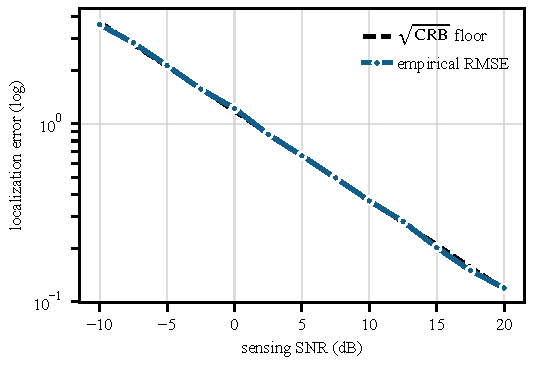
\includegraphics[width=\columnwidth]{fig11_rmse_crb.pdf}
\caption{Empirical localisation RMSE versus the $\sqrt{\mathrm{CRB}}$ floor across SNR (logarithmic axes). The estimator is efficient; the RMSE tracks the bound, so a lower CRB corresponds to better localisation accuracy.}
\label{fig:rmse}
\end{figure}

\subsection{Summary of Findings}
In summary, \scout{} is the most accurate sensing-competitive scheduler in this study on both final and peak accuracy, is Pareto-optimal in $96\%$ of operating points under both CRB conventions, and its gap to the field's best never exceeds $4.7$ percentage points (Fig.~\ref{fig:gapdist}). The lead persists across five datasets, a mid-run budget cut is absorbed within two rounds (Fig.~\ref{fig:adapt}), and the selection overhead is low. \scout{} does not minimise the CRB. Where the sensing requirement is extreme, dedicated sensing methods attain a lower CRB at a substantial accuracy cost.

% ============================================================= VII. CONCLUSION
\section{Conclusion}\label{sec:conclusion}
This paper treated client selection for ISAC over-the-air federated learning as a decision that jointly determines learning and sensing quality, and proposed \scout{}, a scheduler that scores candidate active sets by a geometry-aware submodular utility and respects the AirComp aggregation-MSE budget through a self-tuning primal--dual price. The selector operates as a cognitive control loop that observes the radio environment and the realised aggregation error, decides the active set, and adapts its dual price from the outcome of each round. Greedy selection is $(1-1/e)$-optimal for the composite utility with a curvature refinement, the dual loop is feasible in time average and no-regret, which a mid-run budget cut confirms experimentally, the optimised CRB is empirically achievable, and a convergence bound converts the budget into an explicit guarantee on the trained model. Against eleven sensing-aware baselines, \scout{} attains the highest accuracy of any sensing-competitive method, lies on the accuracy--CRB Pareto frontier in $96\%$ of operating points (Fig.~\ref{fig:gapdist}), and holds its lead across five datasets at a fraction of the overhead of the state of the art. Angular diversity across the active set, rather than raw SNR, is the interpretable mechanism. Future work includes mobile targets with a tracking-aware FIM, multi-antenna clients with beam selection in the greedy step, and joint power control with the dual price.

% ============================================================= APPENDIX
\appendices
\section{Proofs}\label{app:proofs}

\begin{proof}[Proof of Proposition~\ref{prop:submod}]
Consider first the learning utility. Let $\calS\subseteq\calT\subseteq\calN$ and $k\notin\calT$. For every $j\in\calN$, the map $\calS\mapsto\max_{k'\in\calS}s(j,k')$ is monotone non-decreasing, since enlarging the set cannot decrease a maximum, and its marginal gain from adding $k$ is $[\,s(j,k)-\max_{k'\in\calS}s(j,k')\,]_+$, which is non-increasing in the base set because $\max_{k'\in\calS}s(j,k')\le\max_{k'\in\calT}s(j,k')$. Summing over $j$ preserves both properties, so $U_{\mathrm{learn}}$ is monotone submodular.

Consider next the sensing term for a fixed target $m$. Let $F(\calS)=\logdet\bJ_m(\calS)$ with $\bJ_m(\calS)=\bJ_0+\sum_{k\in\calS}\bJ_{k,m}$, $\bJ_0\succ 0$, and $\bJ_{k,m}\succeq 0$. Monotonicity follows because $\bJ_m(\calS\cup\{k\})=\bJ_m(\calS)+\bJ_{k,m}\succeq\bJ_m(\calS)$ and $\logdet$ is monotone with respect to the positive-semidefinite order on the positive-definite cone. For submodularity, let $\calS\subseteq\calT$, write $\bm{A}=\bJ_m(\calS)$ and $\bm{B}=\bJ_m(\calT)$, so that $\bm{B}\succeq\bm{A}\succ 0$, and let $\bm{\Delta}=\bJ_{k,m}\succeq 0$. Define $\phi(s)=\logdet(\bm{A}+s\bm{\Delta})$ for $s\in[0,1]$. Then $\phi'(s)=\tr[(\bm{A}+s\bm{\Delta})^{-1}\bm{\Delta}]$. Since matrix inversion is operator-antitone on the positive-definite cone, $\bm{B}\succeq\bm{A}$ implies $(\bm{B}+s\bm{\Delta})^{-1}\preceq(\bm{A}+s\bm{\Delta})^{-1}$, and therefore, for all $s\in[0,1]$,
\[
\tr\big[(\bm{B}+s\bm{\Delta})^{-1}\bm{\Delta}\big]\;\le\;\tr\big[(\bm{A}+s\bm{\Delta})^{-1}\bm{\Delta}\big].
\]
Integrating over $s\in[0,1]$ yields
\[
\logdet(\bm{B}+\bm{\Delta})-\logdet\bm{B}\;\le\;\logdet(\bm{A}+\bm{\Delta})-\logdet\bm{A},
\]
which is the diminishing-returns inequality. Hence $F$ is submodular, and summing over $m$ preserves monotone submodularity. Finally, a weighted sum of monotone submodular functions with nonnegative weights is monotone submodular, which establishes the claim for $U$ in~\eqref{eq:composite}.
\end{proof}

\begin{proof}[Proof of Proposition~\ref{prop:greedy}]
By Proposition~\ref{prop:submod}, $U$ is monotone submodular with $U(\emptyset)\ge 0$. The claim is the classical guarantee of Nemhauser, Wolsey, and Fisher~\cite{nemhauser1978} for greedy maximisation of a monotone submodular function under a cardinality constraint. Specifically, let $\calS^\star$ denote an optimal set of size $K$ and let $\calS_i$ denote the greedy set after $i$ additions. Monotonicity and submodularity imply
\begin{align*}
U(\calS^\star)&\le U(\calS_i)+\sum_{k\in\calS^\star\setminus\calS_i}\big[U(\calS_i\cup\{k\})-U(\calS_i)\big]\\
&\le U(\calS_i)+K\,\delta_{i+1},
\end{align*}
where $\delta_{i+1}=U(\calS_{i+1})-U(\calS_i)$ is the greedy gain. Rearranging gives $\delta_{i+1}\ge\frac{1}{K}\,[\,U(\calS^\star)-U(\calS_i)\,]$, and by induction
\[
U(\calS^\star)-U(\calS_K)\;\le\;\Big(1-\tfrac{1}{K}\Big)^{K}\,U(\calS^\star)\;\le\;e^{-1}\,U(\calS^\star),
\]
which yields $U(\calS_K)\ge(1-1/e)\,U(\calS^\star)$.
\end{proof}

\begin{proof}[Proof of Proposition~\ref{prop:penalised}]
For part (i), if $\mathrm{MSE}(\calS_t)\le\varepsilon$ holds along the trajectory, then the dual recursion~\eqref{eq:dual} yields $\mu_t=0$ for all $t$, hence $U_{\mu_t}=U$ and the bound of Proposition~\ref{prop:greedy} applies verbatim.

For part (ii), it suffices to exhibit the structural failure. From~\eqref{eq:mse}, $\mathrm{MSE}(\calS)=c/\big(|\calS|^2\min_{k\in\calS}g_k\big)$ with $g_k=|h_k|^2$ and a constant $c>0$. The map $\calS\mapsto\min_{k\in\calS}g_k$ is order-reversing, so $-\mu\,\mathrm{MSE}(\calS)$ is not monotone in $\calS$; moreover, the marginal change in $\mathrm{MSE}$ from adding a client $k$ depends on whether $g_k$ falls below the current minimum, which can make the penalty's marginal \emph{larger} on a larger base set, violating the diminishing-returns inequality. Therefore $U_\mu$ is in general neither monotone nor submodular for $\mu>0$, and the $(1-1/e)$ bound of Proposition~\ref{prop:greedy} does not apply to it. For non-monotone submodular objectives, deterministic greedy selection admits no constant-factor guarantee, and the best known bound of the randomised greedy algorithm is $1/e$~\cite{buchbinder2014}; since $U_\mu$ need not even remain submodular, no constant factor is claimed. Feasibility in this regime is provided by Proposition~\ref{prop:pd}.
\end{proof}

\begin{proof}[Proof of Proposition~\ref{prop:pd}]
Let $v_t=\mathrm{MSE}(\calS_t)-\varepsilon\in[-\varepsilon,\,G-\varepsilon]$ denote the per-round violation, so that the recursion~\eqref{eq:dual} reads $\mu_{t+1}=[\mu_t+\eta v_t]_+$. Squaring and using $([x]_+)^2\le x^2$,
\[
\mu_{t+1}^2\;\le\;\mu_t^2+2\eta\,\mu_t v_t+\eta^2 v_t^2 .
\]
Summing from $t=1$ to $T$ and telescoping with $\mu_1=0$ gives
\[
0\;\le\;\mu_{T+1}^2\;\le\;2\eta\sum_{t=1}^{T}\mu_t v_t+\eta^2\sum_{t=1}^{T}v_t^2 ,
\]
hence $\sum_t \mu_t v_t\ge-\tfrac{\eta}{2}\sum_t v_t^2\ge-\tfrac{\eta}{2}TG^2$. Moreover, the recursion implies $\mu_{t+1}\ge\mu_t+\eta v_t$, so summing yields $\sum_{t=1}^{T}v_t\le\mu_{T+1}/\eta$. The recursion also bounds the dual iterates as $\mu_{t}\le\eta\sum_{s<t}[v_s]_+\le\eta T G$; combining with the drift inequality above and $\eta=\Theta(1/\sqrt{T})$ gives $\mu_{T+1}=O(\sqrt{T}\,\eta\,G)=O(G)$, and therefore
\[
\frac{1}{T}\sum_{t=1}^{T}\big(\mathrm{MSE}(\calS_t)-\varepsilon\big)\;\le\;\frac{\mu_{T+1}}{\eta T}\;=\;O\!\Big(\frac{1}{\sqrt{T}}\Big).
\]
For the regret claim, the recursion~\eqref{eq:dual} is projected online gradient ascent on the concave dual function with bounded subgradients $v_t$; standard online convex optimisation analysis with step size $\eta=\Theta(1/\sqrt{T})$ gives dual regret $O(\sqrt{T})$, and weak duality converts the dual regret into an $O(\sqrt{T})$ cumulative utility gap against the best fixed feasible selection in hindsight.
\end{proof}

\begin{proof}[Proof of Proposition~\ref{prop:crb}]
Under the asymptotic-normality regime of Section~\ref{sec:sensing}, the (range, angle) log-likelihood satisfies the standard regularity conditions for ML asymptotics (differentiability under the integral sign, a nonsingular FIM, and consistency of the estimator)~\cite{kay1993}. It follows that the ML estimator $\hat{\bm{p}}_m$ of target $m$'s position is asymptotically unbiased and asymptotically efficient, i.e.\ $\mathrm{Cov}(\hat{\bm{p}}_m)\to\bJ_m(\calS)^{-1}$ as the observation SNR grows. Therefore the CRB in~\eqref{eq:crb} is attained in this regime, and a difference in CRB between two active sets equals the difference in the asymptotic error covariance of the corresponding estimators. Fig.~\ref{fig:rmse} verifies the finite-sample behaviour.
\end{proof}

\begin{proof}[Proof of Proposition~\ref{prop:learn}]
Write the realised server update as $\bw_{t+1}=\bw_t-\eta_\ell\nabla F(\bw_t)+\bm{\xi}_t+\bm{n}_t$, where $\bm{\xi}_t$ collects the sampling deviation of the aggregated update from its mean and $\bm{n}_t$ is the AirComp noise after post-processing. By (A2), $\mathbb{E}[\bm{\xi}_t\,|\,\bw_t]=0$ and $\mathbb{E}\lVert\bm{\xi}_t\rVert^2\le\eta_\ell^2\sigma_u^2$. The receiver noise is zero mean and independent of $\bw_t$, and by (A3) its contribution to the update error satisfies $\mathbb{E}\lVert\bm{n}_t\rVert^2=\mathrm{MSE}(\calS_t)$. By $L$-smoothness of $F$,
\begin{align*}
F(\bw_{t+1})\le{}& F(\bw_t)+\nabla F(\bw_t)^{\!\top}(\bw_{t+1}-\bw_t)\\
&+\tfrac{L}{2}\lVert\bw_{t+1}-\bw_t\rVert^2 .
\end{align*}
Taking conditional expectations, the cross terms in the inner product vanish, and the quadratic term expands into the three variance contributions. Using $\eta_\ell\le 1/L$ to absorb the gradient part,
\begin{align*}
\mathbb{E}\big[F(\bw_{t+1})\big]\le{}&\mathbb{E}\big[F(\bw_t)\big]-\tfrac{\eta_\ell}{2}\,\mathbb{E}\lVert\nabla F(\bw_t)\rVert^2\\
&+\tfrac{L}{2}\big(\eta_\ell^2\sigma_u^2+\mathrm{MSE}(\calS_t)\big).
\end{align*}
Summing over $t=1,\dots,T$, telescoping against the lower bound $F^\star$, dividing by $\eta_\ell T/2$, and inserting the definition of $\overline{\mathrm{MSE}}_T$ yields~\eqref{eq:learnbound}. The refinement through Proposition~\ref{prop:pd} follows by replacing $\overline{\mathrm{MSE}}_T$ with its guaranteed bound $\varepsilon+O(1/\sqrt{T})$, and the rate statements follow by substituting the indicated choices of $\eta_\ell$ and $\varepsilon$. The argument is the standard descent analysis of stochastic gradient methods under smoothness~\cite{bottou2018}, extended with the additive channel-noise term that the cognitive dual loop controls.
\end{proof}

% ============================================================= REFERENCES
\begin{thebibliography}{99}
\bibitem{liu2022isac} F.~Liu \emph{et al.}, ``Integrated sensing and communications: Toward dual-functional wireless networks for 6G and beyond,'' \emph{IEEE J.\ Sel.\ Areas Commun.}, vol.~40, no.~6, pp.~1728--1767, 2022.
\bibitem{cui2021isac} Y.~Cui, F.~Liu, X.~Jing, and J.~Mu, ``Integrating sensing and communications for ubiquitous IoT: Applications, trends, and challenges,'' \emph{IEEE Network}, vol.~35, no.~5, pp.~158--167, 2021.
\bibitem{mcmahan2017fedavg} B.~McMahan, E.~Moore, D.~Ramage, S.~Hampson, and B.~A.~y~Arcas, ``Communication-efficient learning of deep networks from decentralized data,'' in \emph{Proc.\ AISTATS}, 2017, pp.~1273--1282.
\bibitem{balakrishnan2022divfl} R.~Balakrishnan, T.~Li, T.~Zhou, N.~Himayat, V.~Smith, and J.~Bilmes, ``Diverse client selection for federated learning via submodular maximization,'' in \emph{Proc.\ ICLR}, 2022.
\bibitem{yang2020energy} Z.~Yang, M.~Chen, W.~Saad, C.~S.~Hong, and M.~Shikh-Bahaei, ``Energy efficient federated learning over wireless communication networks,'' \emph{IEEE Trans.\ Wireless Commun.}, vol.~20, no.~3, pp.~1935--1949, 2021.
\bibitem{amiri2021scheduling} M.~M.~Amiri, D.~G\"und\"uz, S.~R.~Kulkarni, and H.~V.~Poor, ``Convergence of update aware device scheduling for federated learning at the wireless edge,'' \emph{IEEE Trans.\ Wireless Commun.}, vol.~20, no.~6, pp.~3643--3658, 2021.
\bibitem{an2026otafl} Q.~An, H.~Zhu, Q.~Ye, N.~Zhang, Y.~Shi, and Y.~Zhou, ``Robust design for RIS-assisted over-the-air federated learning with imperfect cascaded CSI,'' \emph{IEEE Trans.\ Cogn.\ Commun.\ Netw.}, vol.~12, pp.~6045--6060, 2026.
\bibitem{lai2021oort} F.~Lai, X.~Zhu, H.~V.~Madhyastha, and M.~Chowdhury, ``Oort: Efficient federated learning via guided participant selection,'' in \emph{Proc.\ USENIX OSDI}, 2021, pp.~19--35.
\bibitem{li2020fairfl} T.~Li, M.~Sanjabi, A.~Beirami, and V.~Smith, ``Fair resource allocation in federated learning,'' in \emph{Proc.\ ICLR}, 2020.
\bibitem{lai2026cognition} C.-F.~Lai, F.-Y.~Chang, Y.-C.~Chang, and H.-H.~Chen, ``Cognition-driven semi-synchronous federated learning with entropy-aware client scheduling in heterogeneous edge networks,'' \emph{IEEE Trans.\ Cogn.\ Commun.\ Netw.}, vol.~12, pp.~3021--3035, 2026.
\bibitem{chen2024exploring} Z.~Chen, W.~Yi, and A.~Nallanathan, ``Exploring representativity in device scheduling for wireless federated learning,'' \emph{IEEE Trans. Wireless Commun.}, vol.~23, no.~1, pp.~720--735, Jan. 2024.
\bibitem{liu2020beamforming} F.~Liu, C.~Masouros, A.~P.~Petropulu, H.~Griffiths, and L.~Hanzo, ``Joint radar and communication design: Applications, state-of-the-art, and the road ahead,'' \emph{IEEE Trans.\ Commun.}, vol.~68, no.~6, pp.~3834--3862, 2020.
\bibitem{wang2024cramer} Y.~Wang, M.~Tao, and S.~Sun, ``Cram\'er-Rao bound analysis and beamforming design for integrated sensing and communication with extended targets,'' \emph{IEEE Trans.\ Wireless Commun.}, vol.~23, no.~11, pp.~15987--16000, Nov. 2024.
\bibitem{zhou2026crb} J.~Zhou, C.~Zhou, Y.~Sun, and C.~Tellambura, ``CRB-rate tradeoff in RSMA-enabled near-field integrated multi-target sensing and multi-user communications,'' \emph{IEEE Trans.\ Cogn.\ Commun.\ Netw.}, vol.~12, pp.~3687--3700, 2026.
\bibitem{galappaththige2026} D.~Loku~Galappaththige, C.~Tellambura, and S.~P.~Herath, ``Wideband cognitive radio for joint communication and sensing: Optimization of subcarrier allocation and beamforming,'' \emph{IEEE Trans.\ Cogn.\ Commun.\ Netw.}, vol.~12, pp.~1694--1709, 2026.
\bibitem{jiang2026marl} M.~Jiang \emph{et al.}, ``Hierarchical attention-driven multi-agent reinforcement learning for resource allocation in cell-free massive MIMO with integrated sensing and communication,'' \emph{IEEE Trans.\ Cogn.\ Commun.\ Netw.}, vol.~12, pp.~6955--6969, 2026.
\bibitem{wen2023isacfl} D.~Wen \emph{et al.}, ``Task-oriented sensing, computation, and communication integration for multi-device edge AI,'' \emph{IEEE Trans.\ Wireless Commun.}, vol.~23, no.~3, pp.~2486--2502, 2024.
\bibitem{zheng2024otafliscc} P.~Zheng \emph{et al.}, ``Over-the-air federated learning client selection in integrated sensing, computing and communication,'' in \emph{Proc.\ IEEE ICC Workshops}, 2024, pp.~804--809.
\bibitem{du2024fediscc} M.~Du, H.~Zheng, M.~Gao, X.~Feng, J.~Hu, and Y.~Chen, ``Integrated sensing, communication, and computation for over-the-air federated learning in 6G wireless networks,'' \emph{IEEE Internet Things J.}, vol.~11, no.~21, pp.~35551--35567, 2024.
\bibitem{wen2025isccairfeel} D.~Wen, S.~Xie, X.~Cao, Y.~Cui, J.~Xu, Y.~Shi, and S.~Cui, ``Integrated sensing, communication, and computation for over-the-air federated edge learning,'' \emph{IEEE Trans.\ Wireless Commun.}, 2025, to appear (arXiv:2508.15185).
\bibitem{zhang2026isccfl} N.~Zhang, Q.~Hu, D.~Wen, Y.~Mao, T.-M.~Ma, G.~Yu, and W.~Wang, ``Integrated sensing-communication-computation-based online federated learning with limited cache in OFDM systems,'' \emph{IEEE Trans.\ Cogn.\ Commun.\ Netw.}, vol.~12, pp.~5578--5594, 2026.
\bibitem{asaad2025} S.~Asaad, P.~Wang, and H.~Tabassum, ``Over-the-air FEEL with integrated sensing: Joint scheduling and beamforming design,'' \emph{IEEE Trans.\ Wireless Commun.}, 2025, to appear (arXiv:2501.06334).
\bibitem{hu2025differentially} S.~Hu, X.~Yuan, W.~Ni, X.~Wang, E.~Hossain, and H.~V.~Poor, ``Differentially private wireless federated learning with integrated sensing and communication,'' \emph{IEEE Trans.\ Wireless Commun.}, vol.~24, no.~8, pp.~6690--6704, 2025.
\bibitem{mitola1999} J.~Mitola and G.~Q.~Maguire, ``Cognitive radio: Making software radios more personal,'' \emph{IEEE Pers.\ Commun.}, vol.~6, no.~4, pp.~13--18, 1999.
\bibitem{haykin2005} S.~Haykin, ``Cognitive radio: Brain-empowered wireless communications,'' \emph{IEEE J.\ Sel.\ Areas Commun.}, vol.~23, no.~2, pp.~201--220, 2005.
\bibitem{bkassiny2013} M.~Bkassiny, Y.~Li, and S.~K.~Jayaweera, ``A survey on machine-learning techniques in cognitive radios,'' \emph{IEEE Commun.\ Surveys Tuts.}, vol.~15, no.~3, pp.~1136--1159, 2013.
\bibitem{nemhauser1978} G.~L.~Nemhauser, L.~A.~Wolsey, and M.~L.~Fisher, ``An analysis of approximations for maximizing submodular set functions---I,'' \emph{Math.\ Program.}, vol.~14, no.~1, pp.~265--294, 1978.
\bibitem{conforti1984} M.~Conforti and G.~Cornu\'ejols, ``Submodular set functions, matroids and the greedy algorithm: Tight worst-case bounds and some generalizations of the Rado-Edmonds theorem,'' \emph{Discrete Appl.\ Math.}, vol.~7, no.~3, pp.~251--274, 1984.
\bibitem{bottou2018} L.~Bottou, F.~E.~Curtis, and J.~Nocedal, ``Optimization methods for large-scale machine learning,'' \emph{SIAM Rev.}, vol.~60, no.~2, pp.~223--311, 2018.
\bibitem{buchbinder2014} N.~Buchbinder, M.~Feldman, J.~Naor, and R.~Schwartz, ``Submodular maximization with cardinality constraints,'' in \emph{Proc.\ ACM-SIAM SODA}, 2014, pp.~1433--1452.
\bibitem{krause2014submodular} A.~Krause and D.~Golovin, ``Submodular function maximization,'' in \emph{Tractability: Practical Approaches to Hard Problems}.\ Cambridge Univ.\ Press, 2014, pp.~71--104.
\bibitem{kay1993} S.~M.~Kay, \emph{Fundamentals of Statistical Signal Processing: Estimation Theory}.\ Prentice Hall, 1993.
\bibitem{godrich2010} H.~Godrich, A.~M.~Haimovich, and R.~S.~Blum, ``Target localization accuracy gain in MIMO radar-based systems,'' \emph{IEEE Trans.\ Inf.\ Theory}, vol.~56, no.~6, pp.~2783--2803, 2010.
\bibitem{zhang2026integrated} D.~Zhang \emph{et al.}, ``Integrated sensing and communications over the years: An evolution perspective,'' \emph{IEEE Commun.\ Surveys Tuts.}, vol.~28, pp.~5014--5048, 2026.
\end{thebibliography}

\end{document}
